\documentclass[preprint,12pt]{elsarticle}
\usepackage{amsmath,amssymb,graphicx,booktabs,multirow,xcolor,siunitx,microtype,url}
\usepackage[ruled,vlined,linesnumbered]{algorithm2e}
\usepackage[hidelinks]{hyperref}
\usepackage{caption}
\usepackage{float}
\captionsetup{font=small}
\newcommand{\todo}[1]{\textcolor{red}{[TODO: #1]}}   % marked placeholders; search for TODO before submission
\newcommand{\nats}{\,nats}
\DeclareMathOperator{\dirn}{unit}
\DeclareMathOperator{\tr}{tr}
\journal{}
\setlength{\emergencystretch}{3em}

\begin{document}
\begin{frontmatter}
\title{Calibrated Ridge Maps for Token-Embedding Transplantation Across Language Models}

\author[a]{Shibdas Bhattacharya\corref{cor1}}
\ead{23dp0094@iitism.ac.in}
\author[a]{Haider Banka}
\ead{haider@iitism.ac.in}
\cortext[cor1]{Corresponding author.}
\affiliation[a]{organization={Department of Computer Science and Engineering, Indian Institute of Technology (Indian School of Mines)},city={Dhanbad},country={India}}

\begin{highlights}
\item A closed-form, centred, calibrated ridge map initialises new token embeddings
\item Lower NLL than centred official OMP-64 in 23 of 24 expansion comparisons
\item Better than learned initialisers (AweDist, TokDist) in 39 of 40 comparisons
\item Mapping step up to 150 times faster than official OMP-64 on the same device
\item Official OMP fails on GPT-2 receivers unless its inputs are mean-centred
\end{highlights}

\begin{abstract}
Replacing a language model's tokenizer, or adding tokens to it, requires embeddings for tokens the model has never seen. Existing initialisations are heuristic, rely on per-token sparse reconstruction, or need training. We propose a calibrated ridge map: a closed-form ridge regression from donor to receiver embeddings on centred shared tokens, which keeps only the direction of the mapped vector and sets its length with a single calibration against negative log-likelihood (NLL). No gradient is computed. On sentences that contain new domain words, it has a lower NLL than the official orthogonal matching pursuit (OMP) in 23 of 24 paired comparisons with GPT-2 and OPT receivers, and it is significantly better than seven baselines in 78 of 98 comparisons across seven receiver--donor pairs of 125M to 1.5B parameters (74 after Holm correction). It is also better than two learned initialisers, official token distillation and our own hidden-state distillation, in 39 of 40 comparisons, and after fine-tuning it matches the native tokenizer and the best baselines on two classification tasks. Its mapping step is up to 150 times faster than OMP, and the added tokens shorten the sentences that contain them by 3 to 6 per cent. We also show that OMP as shipped fails on GPT-2 receivers unless its inputs are centred.
\end{abstract}

\begin{keyword}
tokenizer transplantation \sep embedding initialisation \sep vocabulary expansion \sep ridge regression \sep orthogonal matching pursuit \sep language models
\end{keyword}
\end{frontmatter}

%% ------------------------------------------------------------------
\section{Introduction}
\label{sec:intro}
A pretrained language model is tied to its tokenizer. When the tokenizer must change, the model needs embeddings for tokens it has never seen. This happens when a general model is adapted to a technical domain by adding frequent domain words as single tokens, when a model is moved to a more efficient or multilingual vocabulary, and when two models with different vocabularies must be merged, ensembled or distilled into one another \cite{goddard2024mergekit,minixhofer2024zett,mundra2024empirical}. Training new embeddings from scratch is costly, and random or mean initialisation is a weak starting point. Several \emph{gradient-free} initialisations have therefore been proposed. The simplest average the receiver embeddings of the pieces a new token splits into \cite{gee2022fvt,hewitt2021initializing}. WECHSEL and FOCUS weight existing embeddings by the similarity of auxiliary static embeddings \cite{minixhofer2022wechsel,dobler2023focus}. Orthogonal matching pursuit (OMP), now the default in the mergekit tokensurgeon tool, writes each new token as a sparse combination of shared tokens in the donor embedding space and applies the same coefficients to the receiver embeddings of those tokens \cite{goddard2025omp,goddard2024mergekit}.

OMP-style reconstruction has two properties that deserve scrutiny. It solves a separate sparse problem for every new token, whose cost grows with the number of new tokens and with the size of the shared vocabulary. It also works in the raw coordinates of the two embedding spaces, which are anisotropic and share a large common mean component \cite{ethayarajh2019contextual,mu2018allbutthetop}. We show that this matters: run exactly as shipped, the official OMP produces new rows that increase the NLL of a GPT-2 receiver by hundreds to thousands of nats, and the failure disappears when the inputs are mean-centred.

We study a simpler alternative. Instead of one sparse problem per token, we fit one linear map from the donor space to the receiver space on the shared tokens (the \emph{anchors}), in closed form with ridge regularisation \cite{hoerl1970ridge}, after centring both spaces. The map predicts a direction in the receiver space. Its length is not trusted, because ridge predictions are shrunk, but set by one calibration: the scale that minimises the NLL of the receiver on a few hundred training sentences. The method is gradient-free: no parameter of the language model is updated and no gradient is computed; the calibration only evaluates the loss.

\paragraph{Contributions}
\begin{enumerate}
\item \textbf{Method.} A closed-form, receiver-calibrated ridge initialiser for new token embeddings (Section~\ref{sec:method}), whose cost depends on the number of new tokens only through one matrix product, and whose mapping step is up to 150 times faster than official OMP-64 on the same device (Section~\ref{sec:speed}).
\item \textbf{Evidence in vocabulary expansion.} In 12 real vocabulary-expansion runs (four pairs, three seeds), ridge has a lower NLL than official OMP-64 with centred inputs in 23 of 24 paired comparisons, and in all 24 when OMP uses the same calibrated length (Section~\ref{sec:realvocab}). On seven PubMed pairs from 125M to 1.5B parameters it is significantly better than seven baselines in 78 of 98 comparisons and significantly worse in one (Section~\ref{sec:scale}).
\item \textbf{Comparison with learned initialisers.} Ridge is better than official token distillation (AweDist) and our hidden-state distillation (TokDist) in 39 of 40 comparisons on five pairs, without training on any text (Section~\ref{sec:learned}).
\item \textbf{A baseline failure and its repair.} Official OMP as shipped fails on GPT-2 receivers; centring its inputs repairs it.
\item \textbf{Analysis.} Ablations show which components matter (Section~\ref{sec:ablation}); regularisation matters when anchors are scarce (Section~\ref{sec:scarce}), whereas with many anchors the gain comes from fitting on the most frequent ones (Section~\ref{sec:control}); and the added tokens shorten the sentences that contain them by 3 to 6\,\% (Section~\ref{sec:seqlen}).
\end{enumerate}

\section{Related work}
\label{sec:related}
\paragraph{Heuristic initialisation} Initialising a new token with the mean of the receiver embeddings of its pieces is the common default \cite{gee2022fvt,hewitt2021initializing}; Mundra et al.\ compare several such schemes for vocabulary expansion \cite{mundra2024empirical}. They ignore the geometry of the donor model and place new tokens near the centre of the receiver space, which we reproduce as a baseline with a calibrated length.

\paragraph{Similarity-based transfer} WECHSEL initialises subword embeddings for a new language from a softmax-weighted combination of the nearest source tokens, found in an aligned static embedding space \cite{minixhofer2022wechsel}. FOCUS uses the same principle for tokens absent from the source vocabulary, with a fastText model trained on target data \cite{dobler2023focus,bojanowski2017fasttext}. Both use auxiliary static embeddings and do not use the weights of a donor language model. OFA factorises the embedding matrix and initialises unseen subwords from well-aligned multilingual static embeddings \cite{liu2024ofa}, and CLP-Transfer and trans-tokenization initialise target-language embeddings from those of similar tokens in a smaller same-family model or from a parallel-corpus token alignment \cite{ostendorff2023clptransfer,remy2024transtokenization}. These methods rely on auxiliary resources (static embeddings, a helper model or parallel text), which our setting does not assume; we do not compare against them.

\paragraph{Reconstruction-based transfer} OMP \cite{pati1993omp,tropp2007signal} approximates a target vector by a sparse combination of dictionary atoms. Goddard and Fernandes Neto apply it to tokenizer transplantation: each new token is reconstructed from shared tokens in the donor space, and the coefficients are applied to the receiver embeddings \cite{goddard2025omp}. It is implemented in mergekit \cite{goddard2024mergekit}. We use this official implementation as our main baseline.

\paragraph{Regression-based transfer}SALT fits a separate linear regression for each non-overlapping token on its semantically similar shared tokens \cite{lee2025salt}. Our map differs in being one global map fitted once on all (or the most frequent) anchors, which is what makes its cost nearly independent of the number of new tokens. We could not identify an official SALT implementation, so Section~\ref{sec:scale} uses SALT-ours, a simplified local-regression baseline in its spirit; it is our adaptation, not the method of Lee et al.\par\paragraph{Learned approaches} Zero-shot tokenizer transfer trains a hypernetwork that predicts embeddings for any tokenizer \cite{minixhofer2024zett}. Token distillation learns new input embeddings by matching the hidden states of the original model \cite{dobler2025tokendistillation}, and TokAlign learns a token alignment between vocabularies \cite{li2025tokalign}. These approaches need additional training, whereas the method here is closed form. We compare against token distillation, using the authors' code (AweDist) and our own simplified re-implementation (TokDist), in Section~\ref{sec:learned}; we do not compare against the hypernetwork of ZeTT or TokAlign.

\paragraph{Linear maps between embedding spaces} Fitting a linear map between two embedding spaces on a seed dictionary is a standard tool in cross-lingual word embeddings \cite{mikolov2013exploiting}. Our map is of this kind, with two changes that matter here: both spaces are centred, and the length of the predicted vector is calibrated on the receiver model rather than taken from the regression.

\section{Method}
\label{sec:method}
\subsection{Problem}
Let a receiver model $R$ with tokenizer $\mathcal T_r$ and embedding matrix $E_r\in\mathbb R^{|\mathcal V_r|\times d_r}$ receive new tokens whose embeddings must be built, and let a donor model $D$ with tokenizer $\mathcal T_d$ and embedding matrix $E_d\in\mathbb R^{|\mathcal V_d|\times d_d}$ define them. In \emph{tokenizer transplantation} the receiver adopts the donor tokenizer, tokens present in both vocabularies keep the receiver embedding, and every other donor token needs a new row. In \emph{vocabulary expansion} the receiver keeps its own vocabulary and gains new tokens, here whole words that the receiver splits into two or more pieces and the donor holds as one token. We call tokens whose string occurs in both vocabularies \emph{anchors}, with embeddings $X\in\mathbb R^{n\times d_d}$ (donor) and $Y\in\mathbb R^{n\times d_r}$ (receiver). Let $x_*\in\mathbb R^{d_d}$ be the donor embedding of a new token. The goal is a row $\hat y_*\in\mathbb R^{d_r}$ for the receiver.

\subsection{Calibrated ridge map}
\paragraph{Centring} Let $\mu_d$ and $\mu_r$ be the means of \emph{all} anchors, $X_c=X-\mu_d$ and $Y_c=Y-\mu_r$. Embedding spaces share a large common mean component, and a map fitted in raw coordinates has to reproduce it for every token. We fit in centred coordinates and add $\mu_r$ back. The means and the mean receiver norm $\bar r$ below always come from all anchors, also when the map is fitted on a subset (next subsection). The donor side is divided by the mean row norm $s=\frac1m\sum_i\|X_{c,i}\|$ of the $m$ centred anchors used to fit the map; $s$ only fixes the scale of $\lambda$ and does not change the direction.

\paragraph{Ridge direction} With $\tilde X=X_c/s$ we solve
\begin{equation}
W=\bigl(\tilde X^\top\tilde X+\lambda\,\tfrac{\tr(\tilde X^\top\tilde X)}{d_d}I\bigr)^{-1}\tilde X^\top Y_c ,
\label{eq:ridge}
\end{equation}
Here $s$ is the mean norm of the centred fitting anchors, which only puts $\tilde X$ on unit scale. Because the penalty is relative ($\lambda$ times the mean diagonal of $\tilde X^\top\tilde X$), replacing $s$ by any other constant changes $W$ by the inverse factor and leaves the direction $u_*$ in Eq.~\eqref{eq:dir} unchanged. The strength $\lambda$ is chosen from $\{10^{-4},10^{-3},10^{-2},10^{-1},1\}$ by the mean cosine similarity between the predicted and the true \emph{centred} receiver rows on held-out anchors (10\,\% of the fitting anchors, at least 50 and at most 20\,\%; for each $\lambda$ the map is fitted on the remaining anchors, and it is refitted on all fitting anchors with the chosen $\lambda$). We select $\lambda$ by cosine on held-out anchors because $\lambda$ governs how well the map generalises from anchors to other tokens, which can be measured on anchors alone and needs no forward pass of the language model. The length cannot be learned this way, because regression shrinks norms and the right length depends on how the receiver model uses the new row, so we calibrate it on NLL (below). The direction of a new token is
\begin{equation}
u_*=\dirn\!\bigl(\tfrac{x_*-\mu_d}{s}\,W\bigr),\qquad \dirn(v)=v/\|v\|.
\label{eq:dir}
\end{equation}

\paragraph{Calibrated length} Regression shrinks predictions, so the norm of $\tfrac{x_*-\mu_d}{s}W$ is not a reliable length. We set
\begin{equation}
\hat y_*=\mu_r+c\,\bar r\,u_*,\qquad \bar r=\tfrac1n\sum_i\|Y_{c,i}\|,
\label{eq:row}
\end{equation}
where $\bar r$ is the mean norm of the centred receiver anchors and $c$ is a single scalar for all new tokens, chosen from $\{0.3,0.5,0.6,0.7,0.8,0.9,1.0,1.2,1.5\}$ to minimise the receiver's negative log-likelihood on a few hundred \emph{training} sentences (Section~\ref{sec:setup}). The calibration changes no parameter of the language model other than the new rows. In the 17 runs of Section~\ref{sec:results} (51 selections for ridge[all], ridge[freq5000] and centred OMP-64), the selected $c$ was never at the edge of the grid (0.3 or 1.5): it ranged from 0.6 to 1.2.

\paragraph{Relation to least squares} Our least-squares baseline uses the same centred anchors, the same direction-only normalisation and the same calibrated length as ridge, so ridge differs from it in two choices only: the penalty $\lambda$ (chosen by held-out cosine) and, for the variant fitted on the 5000 most frequent anchors, the anchor subset. Section~\ref{sec:control} separates the two. With many anchors the subset accounts for the gain over least squares and the penalty makes no consistent difference; the penalty matters when the number of anchors is small relative to the embedding dimension, where least squares collapses (Section~\ref{sec:scarce}). Ridge is therefore best described as a frequency-selected linear map with a calibrated length, fitted by a stable estimator.
\subsection{Anchor subset and selection}
We fit Eq.~\eqref{eq:ridge} twice, on all anchors and on the 5000 most frequent anchors (frequency of the anchor token in the training text), calibrate each, and keep the one with the lower training objective. The selection uses only training data. We call the two variants ridge[all] and ridge[freq5000] and the selected one ridge[sel]; the tables report ridge[sel] unless stated.

\paragraph{Untied receivers}\label{par:untied} If the receiver has separate input and output embedding matrices, the procedure is run twice: the input matrix with the donor input embeddings, and the output matrix with the donor output embeddings (the input embeddings if the donor ties them). Each side has its own $\mu_r$, $\bar r$ and map, and one scalar $c$ is shared and calibrated on the NLL with both matrices set.

\begin{algorithm}[t]
\caption{Calibrated ridge initialisation}
\label{alg:ridge}
\KwIn{anchor embeddings $X,Y$; donor embeddings $x_*$ of the $K$ new tokens; calibration sentences}
\KwOut{rows $\hat y_*$ for the $K$ new tokens}
\For{each anchor subset $S\in\{\text{all},\ \text{5000 most frequent}\}$}{
  centre $X_S,Y_S$ with the means $\mu_d,\mu_r$ of all anchors; scale by the mean norm $s$ of the centred $X_S$\;
  choose $\lambda$ on held-out anchors by cosine; solve Eq.~\eqref{eq:ridge}\;
  compute directions $u_*$ by Eq.~\eqref{eq:dir}\;
  choose $c$ on the grid by the receiver NLL on the calibration sentences; set rows by Eq.~\eqref{eq:row}\;
}
\Return the rows of the subset with the lower calibration objective\;
\end{algorithm}

\subsection{Cost}
For $m$ fitting anchors and $K$ new tokens, one dense primal ridge fit followed by the prediction costs
\begin{equation}
O(m d_d^2) + O(m d_d d_r) + O(d_d^3) + O(d_d^2 d_r) + O(K d_d d_r),
\end{equation}
which covers, in order, the donor Gram matrix $\tilde X^\top\tilde X$, the cross-covariance $\tilde X^\top Y_c$, the factorisation of the $d_d\times d_d$ system, the solve with $d_r$ right-hand sides, and the prediction (one product with $W$ per new token, $O(d_d d_r)$). This is the computation specified by Eq.~\eqref{eq:ridge}, not a different method. Only the last term depends on $K$. The $\lambda$ search adds five such fits on 90\,\% of the anchors (without the prediction term) and one final fit, for each of the two anchor subsets, a constant number of solves per receiver--donor pair; the subset selection and the length calibration (below) add further work that is independent of $K$ in the first case and of the mapping step in the second. The official batch OMP of mergekit, as implemented, correlates the residual of every new token with all $n$ anchors in each of $k$ iterations, $O(k\,n\,d_d)$ per token, plus $O(k^2 d_d)$ for the orthogonalisation and $O(k\,d_r)$ to apply the coefficients. Variants that precompute the $n\times n$ Gram matrix of the anchors move part of this cost into a one-off $O(n^2 d_d)$ step; we did not time such variants. Ridge cost is therefore almost independent of $K$ after a one-off fit, and OMP cost is linear in $K$ (Section~\ref{sec:speed}); for small $K$ the one-off fit dominates, and with the $\lambda$ search ridge is no faster than OMP-64 at $K=82$. The length calibration needs $|\mathcal C|=9$ forward passes over the calibration sentences; it is required by every calibrated method and is not part of the mapping step.

\section{Experimental setup}
\label{sec:setup}
\subsection{Models and data}
Receivers are GPT-2 small, medium and large \cite{radford2019gpt2}, OPT-125m \cite{zhang2022opt} and Qwen2.5-0.5B \cite{qwen2024qwen25}; donors are Pythia-160m \cite{biderman2023pythia}, Qwen2.5-0.5B and GPT-2. Domain text is PubMed abstracts (PubMedQA contexts \cite{jin2019pubmedqa}, 4000 abstracts); general text is WikiText-2 \cite{merity2017pointer}. Abstracts are split 70/30 by abstract into training and evaluation text. Sentences have 8 to 60 words. All NLL values are the \emph{total} NLL of a sentence in nats, which is comparable across tokenizers.

\subsection{Three evaluation settings}
\paragraph{Tokenizer swap (zero-shot)} A receiver keeps its weights and adopts the donor tokenizer (GPT-2$\leftarrow$Pythia, GPT-2$\leftarrow$Qwen2.5, GPT-2 medium$\leftarrow$Pythia, Qwen2.5$\leftarrow$GPT-2). Tokens in both vocabularies keep the receiver row (these are the anchors), all others are filled by each method. We report the NLL of 400 PubMed and 400 WikiText-2 evaluation sentences, with 150 sentences of each type from the training text for calibration. The unchanged model with its own tokenizer is a reference only, because its tokenisation differs.

\paragraph{Real vocabulary expansion}\label{par:rvprotocol} New tokens are domain words. A word is eligible if it is alphabetic with at least 4 letters, occurs at least 5 times in the \emph{training} text, is split into two or more pieces by the receiver and is a single token of the donor. Eligible words are ranked by their frequency in the training text (ties alphabetically) and the top 300 are kept, so the selection uses neither the evaluation text nor any initialisation method; 52 to 300 words qualify per pair. Anchors are whole words (tokens with a leading space, alphabetic, at least 3 letters) present in both vocabularies. Each new word becomes one new token of the receiver. Sentences containing a new word are scored zero-shot and after \emph{200 steps in which only the new embedding rows are trained} (AdamW, learning rate $10^{-3}$, no weight decay, batches of 8 training sentences containing new words; the model and all old rows stay frozen, the output matrix is tied to the input matrix). The reference is the unchanged receiver, where the word stays split. Calibration uses 300 training sentences containing new words and 150 control sentences. Evaluation uses 600 sentences containing new words and two control sets of 200. Receivers are GPT-2 and OPT-125m, donors Pythia-160m and Qwen2.5-0.5B. We ran PubMed text with seeds 0, 1 and 2 (12 runs). A second text domain, arXiv abstracts (3621 abstracts of at least 600 characters from eight categories, collected through the arXiv API; Section~\ref{sec:arxiv}), was run with the same protocol for the four small pairs on seed 0; there 199 to 300 words qualify per pair. The seed controls the sample of calibration, training and evaluation sentences (all eligible sentences are used when fewer than the requested number exist) and the order of the training batches; the held-out split used to choose $\lambda$ is fixed, and the words, the 70/30 text split and the anchors do not change, so the seeds resample sentences from the same abstracts and are not independent datasets.

\paragraph{Larger receivers}\label{par:large} The protocol above is repeated for PubMed with GPT-2 large (0.77B, tied) $\leftarrow$ Qwen2.5-0.5B (126 words), Pythia-1B (untied) $\leftarrow$ Qwen2.5-0.5B (52 words) and Qwen2.5-1.5B (tied) $\leftarrow$ Pythia-410m (300 words), and, on the four small pairs, with the extra baselines of this paper. The eligibility rule is the same for all pairs. Pythia's tokenizer splits few medical words, so only 52 words qualify for Pythia-1B, with 89 evaluation sentences from 69 abstracts. Pythia-1B is untied and follows the procedure of Section~\ref{par:untied}; training then updates the new rows of both matrices, and the old rows are restored exactly afterwards. For Qwen2.5-1.5B the 200 training steps use gradient accumulation in micro-batches of 2, which is equivalent to a batch of 8. The tables of Sections~\ref{sec:scale} and~\ref{sec:learned} use seed 1 for all seven pairs; GPT-2 large and Pythia-1B were also run with seed 0, and Qwen2.5-1.5B was run once.

\paragraph{Downstream classification} PubMed 20k RCT \cite{dernoncourt2017pubmedrct}, five sentence classes, 2000 training and 2000 test sentences. \emph{Fine-tuning:} all weights of the transplanted GPT-2 are trained for 3 epochs (AdamW \cite{loshchilov2019adamw}, learning rate $2\times10^{-5}$, weight decay 0.01, 10\,\% warm-up, linear decay, batch 16, maximum length 96) on mean-pooled hidden states with a new linear head (learning rate $10^{-3}$); 3 seeds for GPT-2$\leftarrow$Qwen2.5 and 5 for GPT-2$\leftarrow$Pythia. \emph{Frozen probe:} the transplanted model is frozen, and a logistic regression ($C=0.1$) is trained on mean-pooled features of the embedding layer, the middle layer and the last layer; five training subsets of 2000 sentences from a pool of 6000, the same for every method, and the same 2000 test sentences (majority-class accuracy 0.334). \emph{Second task:} medical abstracts \cite{schopf2022evaluating}, five disease classes (neoplasms, digestive system, nervous system, cardiovascular, general pathological conditions), 2000 training and 1000 test abstracts sampled from the released split (majority-class accuracy 0.351). The transplanted GPT-2 is fine-tuned as above with a maximum length of 128 tokens, for 3 seeds, on GPT-2$\leftarrow$Pythia-160m and GPT-2$\leftarrow$Qwen2.5-0.5B; the methods are ridge, official OMP-64 (as shipped and with centred inputs), FOCUS, the subword mean, mean fill and the native tokenizer.

\subsection{Baselines}
All baselines use the same new tokens and the same evaluation. We use the \emph{official} implementations: \textbf{OMP-64} (the default) and OMP-32 through mergekit-tokensurgeon, and its subword-mean, mean, John Hewitt and common-interpolation methods \cite{goddard2024mergekit}; \textbf{FOCUS} through the \texttt{deepfocus} package, with a fastText model of minimum count 10 trained on up to 60\,000 training sentences \cite{dobler2023focus}. Because OMP as shipped works in raw coordinates, we also run it on mean-centred inputs: both embedding tables are shifted by their anchor means, the official function is applied unchanged, and the receiver mean is added back to the output. For real vocabulary expansion we call the official \texttt{batch\_omp} function (copied from mergekit 0.1.5) with $k=64$ on the receiver anchor rows, as the tool does, and we also run our own scikit-learn OMP with $k=32$ on centred inputs and a mean-of-pieces baseline. The latter two use the calibrated length of Eq.~\eqref{eq:row} and are labelled as our implementations. \textbf{WECHSEL} through the official package \texttt{wechsel} 0.0.4 \cite{minixhofer2022wechsel}, run in same-language mode: the same English fastText model (cc.en.300.bin) serves as source and target embedding, no alignment is applied (\texttt{align\_strategy=None}), with the default 10 neighbours and temperature 0.1; the receiver is the source model and the donor tokenizer is the target. We report it with its own output length (raw) and with the calibrated length of Eq.~\eqref{eq:row}. WECHSEL was run for real vocabulary expansion on PubMed text, seed 1, four pairs (no fallback to a default row was needed); it was not run in the other settings. \textbf{AweDist}, the official token distillation \cite{dobler2025tokendistillation}, is run with the authors' code (commit \texttt{bbd64cc}) on tied receivers: learning rate $10^{-4}$, one epoch, 5 snippets per word (lowered from 25 because our text has few occurrences of each word), full precision, with the official script's document budget of 7000 PubMed abstracts, which are our training abstracts plus further PubMedQA abstracts that are never used for evaluation. \textbf{TokDist} is \emph{our} simplified re-implementation of the same idea, not the authors' code: each new input row, initialised at the mean of the word's receiver pieces, is trained to make the last-layer hidden states of the unchanged receiver at the new token and the following 12 segments equal those it produces on the original pieces (mean-squared error, 25 training contexts per word, 3 epochs, batch 32, learning rate chosen from $\{3\times10^{-4},10^{-3},3\times10^{-3}\}$ on 10\,\% held-out contexts). Each learned row set is also reported with the calibrated length of Eq.~\eqref{eq:row} (``cal.''), applied to its direction. The downstream experiments also use mean fill (every new row set to the anchor mean) as a floor. Three further baselines are \emph{our adaptations}, not official implementations, and are used only in Section~\ref{sec:scale}: \textbf{LS} (minimum-norm least squares on the centred anchors, no regularisation), \textbf{Procrustes} (the partial isometry from the SVD of the centred cross-covariance) and \textbf{SALT-ours} (for each new token, a ridge regression with intercept, $\lambda=10^{-2}$ relative, fitted on its 2000 nearest anchors in the donor space, in the spirit of SALT \cite{lee2025salt}). Each is reported with the calibrated length of Eq.~\eqref{eq:row} (``cal.''); SALT-ours is also reported with its own length (``raw'').

\subsection{Statistics}
\label{sec:stats}
Differences between two methods are paired over sentences (or test items) and summarised by the mean with a 95\,\% percentile bootstrap interval. For real vocabulary expansion (all 17 runs of Sections~\ref{sec:realvocab}--\ref{sec:learned}) the bootstrap resamples \emph{abstracts}, taking all evaluation sentences of a drawn abstract together, and the mean is taken over the resampled sentences; the abstracts were recovered by rebuilding the sampling and checked against the stored token counts (\ref{app:repro}). Other tables (fine-tuning, frozen probe, ablation, anchors) resample test items; real vocabulary expansion and the frozen probe use 5000 resamples (the arXiv and control tables of Sections~\ref{sec:arxiv} and~\ref{sec:control} use 20\,000), the medical-abstracts task 100\,000 and the other tables 2000, and fine-tuning pools the paired differences over seeds. We call an interval that excludes 0 significant. The 54 frozen-probe comparisons (six baselines in nine cells) are additionally corrected with the Holm procedure \cite{holm1979simple} using bootstrap $p$-values. The other tables are \emph{not} corrected for multiple comparisons, and we read them for consistency across pairs, not for single cells. Because tokenisations differ, we also give bits per byte: the mean paired NLL difference divided by $\ln 2$ and by the mean number of UTF-8 bytes per evaluation sentence (about 160 to 170; \ref{app:bpb}).

\paragraph{Multiplicity} Besides the 54 frozen-probe tests, we apply Holm's procedure to the 24 comparisons of ridge with centred OMP-64 in the 12-run set (and separately with its calibrated-length version), to the 98 comparisons of Section~\ref{sec:scale} (seven baselines, 14 each; the comparisons with the unchanged receiver are descriptive and not in this family), to the 168 comparisons of the same seven baselines in the four small pairs with all three seeds, to the 40 comparisons with learned initialisers (Section~\ref{sec:learned}), to the 56 comparisons of the arXiv runs (four pairs, six baselines and the unchanged receiver, zero-shot and after training; Section~\ref{sec:arxiv}), separately for each of the three columns to the eight comparisons of the least-squares control (Section~\ref{sec:control}) and to the five comparisons of the 7B run (Section~\ref{sec:7b}) and, separately for the first and for the last epoch, to the 10 comparisons of ridge with five baselines in each medical-abstracts run set (Section~\ref{sec:downstream}). These $p$-values are two-sided and come from a normal approximation to the bootstrap distribution (standard error from 5000 resamples of abstracts); a comparison counts as significant in the text when its 95\,\% percentile interval excludes 0, and as surviving the correction when its Holm-adjusted $p$-value is below 0.05. Other tables remain uncorrected.


\paragraph{Dependence} Sentences from the same abstract are not independent, so the PubMed intervals resample abstracts. This widened the standard errors by a median of 6\,\% (600 sentences come from 394 to 454 abstracts; the 89 sentences of Pythia-1B come from 69), so the clustering matters little here. Sentences that share a new word are also dependent, and we did not resample by word. We read single intervals cautiously and rely on consistency across runs and pairs. The unit closest to independent is the receiver--donor pair (four in the 12-run set, seven in Section~\ref{sec:scale}), too few for a pair-level test. Seeds resample sentences and training batches only, so they are repeated measures, not independent replicates.

\section{Results}
\label{sec:results}
\subsection{Zero-shot tokenizer swap}
Table~\ref{tab:zs} and Fig.~\ref{fig:zs} give the NLL after swapping the tokenizer without any training.
\begin{table}[t]
\centering\small
\caption{Zero-shot sentence NLL (nats, lower is better) after a tokenizer swap. Dom = PubMed, Gen = WikiText-2. Bold = best transplant method per column. $^{\dagger}$Reference only: a different tokenisation, not a like-for-like comparison.}
\label{tab:zs}
\resizebox{\textwidth}{!}{\begin{tabular}{lrrrrrrrr}
\toprule
 & \multicolumn{2}{c}{GPT-2$\leftarrow$Pythia} & \multicolumn{2}{c}{GPT-2$\leftarrow$Qwen2.5} & \multicolumn{2}{c}{GPT-2 med.$\leftarrow$Pythia} & \multicolumn{2}{c}{Qwen2.5$\leftarrow$GPT-2} \\
\cmidrule(lr){2-3}\cmidrule(lr){4-5}\cmidrule(lr){6-7}\cmidrule(lr){8-9}
Method & Dom & Gen & Dom & Gen & Dom & Gen & Dom & Gen \\
\midrule
Unchanged model (own tokenizer)$^{\dagger}$ & 124.3 & 133.2 & 124.3 & 133.2 & 113.6 & 125.4 & 106.4 & 121.4 \\
\midrule
OMP-64, as shipped & 7711.0 & 7343.8 & 3682.8 & 3364.4 & 6565.0 & 6147.1 & 129.8 & 129.1 \\
OMP-64, centred inputs & 135.8 & 142.3 & 163.0 & 161.2 & 127.8 & 134.8 & \textbf{128.5} & \textbf{128.1} \\
FOCUS & 144.9 & 144.0 & 179.1 & 170.3 & 141.5 & 137.3 & 165.3 & 159.6 \\
Subword mean & 146.6 & 148.9 & 192.0 & 186.7 & 136.8 & 139.9 & 171.4 & 157.9 \\
Mean & 155.4 & 144.2 & 187.5 & 167.3 & 150.2 & 137.6 & 226.9 & 219.8 \\
John Hewitt & 159.1 & 150.3 & 200.7 & 184.3 & 154.3 & 142.7 & 149.4 & 144.1 \\
Common interpolation & 157.8 & 144.3 & 182.8 & 164.9 & 151.1 & 137.4 & 138.4 & 134.0 \\
Ridge, uncalibrated length & 137.2 & 142.1 & 161.7 & 159.9 & 129.5 & 134.7 & 131.1 & 129.0 \\
\textbf{Ridge, calibrated (ours)} & \textbf{135.0} & \textbf{142.0} & \textbf{159.5} & \textbf{159.6} & \textbf{127.6} & \textbf{134.5} & 130.3 & 128.2 \\
\bottomrule
\end{tabular}
}
\end{table}
\begin{figure}[t]
\centering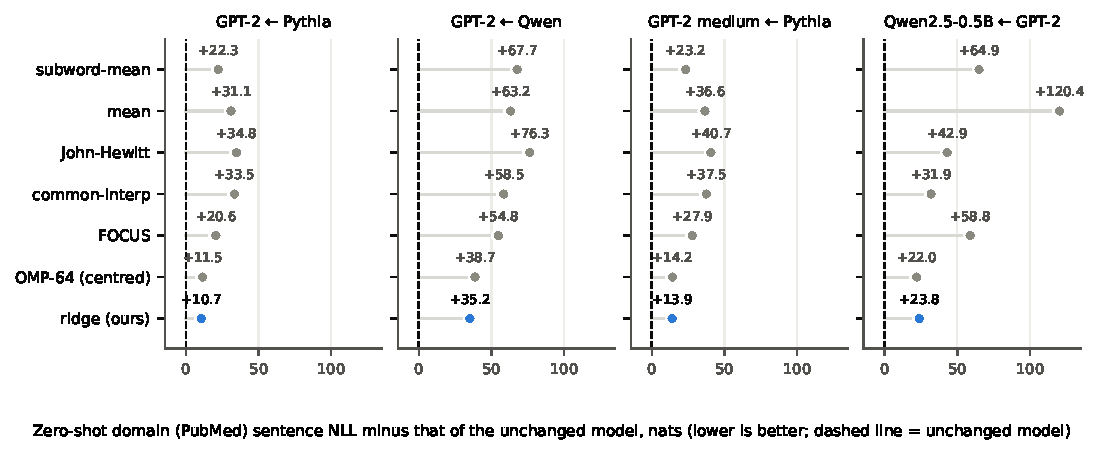
\includegraphics[width=0.95\textwidth]{figures/fig2_zero_shot_nll.pdf}
\caption{Domain (PubMed) NLL by method for each pair. OMP-64 as shipped (3.7k--7.7k nats on GPT-2 receivers) is omitted from the plot and listed in Table~\ref{tab:zs}. The dashed line is the unchanged model with its own tokenizer.}
\label{fig:zs}
\end{figure}
On the three GPT-2-receiver pairs, calibrated ridge has the lowest NLL of all methods on both text types. It is 10 to 20 nats below FOCUS and 9 to 33 nats below the subword mean on domain text. Against OMP-64 with centred inputs the margins are small. The paired difference ridge minus centred OMP-64 is $-0.85$ nats (95\,\% CI $-1.27$ to $-0.42$) on GPT-2$\leftarrow$Pythia and $-3.53$ ($-4.08$ to $-3.01$) on GPT-2$\leftarrow$Qwen2.5 on domain text, $-0.30$ ($-0.75$ to $+0.21$) on GPT-2 medium$\leftarrow$Pythia, and $+1.82$ ($+1.32$ to $+2.34$) on Qwen2.5$\leftarrow$GPT-2, where centred OMP-64 is significantly better. On general text the differences are $-0.33$, $-1.60$ and $-0.24$ (all significant) for the GPT-2 receivers and $+0.14$ ($-0.25$ to $+0.52$) for Qwen2.5. OMP-64 as shipped is catastrophic on the GPT-2 receivers (3.4k to 7.7k nats) and merely worse on Qwen2.5 ($129.8$ vs.\ $128.5$ nats); the uncalibrated ridge length is 0.1 to 2.2 nats worse than the calibrated one (Table~\ref{tab:zs}). Centring is therefore the difference between a working and a failing OMP on GPT-2 receivers, and we use the centred version as the strongest baseline throughout.

\subsection{Real vocabulary expansion}
\label{sec:realvocab}
Table~\ref{tab:rv} summarises the 12 runs and Fig.~\ref{fig:rv} shows each run against centred OMP-64; the full per-run table is in \ref{app:rv}.
\begin{table}[t]
\centering\small
\caption{Real vocabulary expansion, 12 runs (PubMed seeds 0--2, four receiver--donor pairs). Difference in sentence NLL (nats) of ridge minus each method; negative = ridge better. Median and range over runs; CI$<0$ = number of runs whose 95\,\% bootstrap interval lies below 0. ``Calibrated length'' uses the same length rule as ridge, isolating the direction. The last two rows compare ridge with the unchanged receiver (word left split). WECHSEL is reported separately in Table~\ref{tab:wech}.}
\label{tab:rv}
\resizebox{\textwidth}{!}{\begin{tabular}{lrrrrrr}
\toprule
 & \multicolumn{3}{c}{Zero-shot} & \multicolumn{3}{c}{After 200 steps} \\
\cmidrule(lr){2-4}\cmidrule(lr){5-7}
Ridge minus & Median & Range & CI$<0$ & Median & Range & CI$<0$ \\
\midrule
OMP-64, centred inputs (official) & $-$2.14 & $-$3.23 to $-$1.25 & 12/12 & $-$0.56 & $-$0.84 to $-$0.05 & 11/12 \\
OMP-64, centred, calibrated length & $-$1.30 & $-$1.50 to $-$1.02 & 12/12 & $-$0.57 & $-$0.73 to $-$0.45 & 12/12 \\
OMP-64, as shipped (official) & $-$230 & $-$3526 to $-$1.02 & 12/12 & $-$0.64 & $-$96.6 to $-$0.48 & 12/12 \\
OMP-32, centred (our scikit-learn) & $-$0.90 & $-$1.20 to $-$0.23 & 12/12 & $-$0.44 & $-$0.64 to $-$0.19 & 11/12 \\
Mean of word pieces (calibrated) & $-$5.99 & $-$8.87 to $-$4.84 & 12/12 & $-$1.83 & $-$2.64 to $-$1.11 & 12/12 \\
\midrule
\multicolumn{7}{l}{Zero-shot, ridge vs.\ unchanged receiver: better in 0, level in 3, worse in 9 of 12 runs} \\
\multicolumn{7}{l}{After 200 steps, ridge vs.\ unchanged receiver: better in 9, level in 2, worse in 1 of 12 runs} \\
\bottomrule
\end{tabular}
}
\end{table}
\begin{figure}[t]
\centering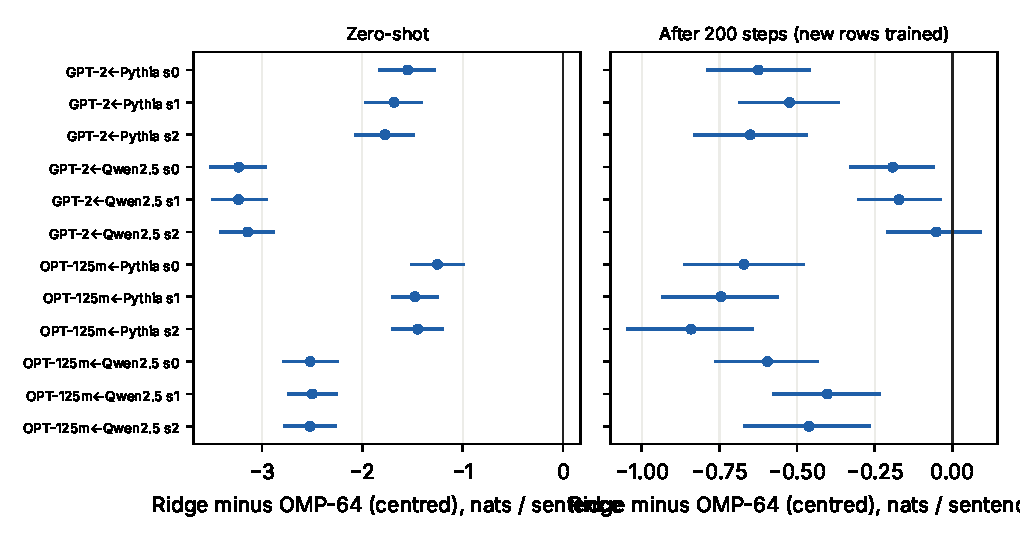
\includegraphics[width=0.85\textwidth]{figures/fig_realvocab.pdf}
\caption{Ridge minus official OMP-64 with centred inputs for each run (point: difference in NLL per sentence, bar: 95\,\% bootstrap interval; negative = ridge better).}
\label{fig:rv}
\end{figure}
Ridge has a lower NLL than centred OMP-64 in 23 of 24 comparisons with the interval excluding 0 (the exception is one run after training the new rows), and all 23 remain significant after Holm correction; against OMP-64 with the same calibrated length ridge is better in all 24, all of them significant after the correction. The margin against centred OMP-64 is 1.3 to 3.2 nats zero-shot and 0.05 to 0.84 after training the new rows. Even when OMP is given the same calibrated length as ridge, the margin is 1.0 to 1.5 nats zero-shot and 0.5 to 0.7 after training, so the advantage is not only a matter of length: it lies in the direction. Ridge is also better than our sparse OMP-32 in all 12 runs zero-shot and in 11 after training, and than the mean of word pieces in all 24 comparisons. The 24 comparisons come from 12 runs that share words and abstracts, so they are not 24 independent tests: the number of independent units is closer to four (the receiver--donor pairs) than to 24. The mean difference is negative in all four pairs, zero-shot and after training. OMP-64 as shipped is far worse on GPT-2 receivers with the Pythia donor ($-3526$ to $-3179$ nats zero-shot for the ridge difference) and with the Qwen donor ($-477$ to $-458$).

Against the unchanged receiver, ridge is not uniformly better. Zero-shot, it is better in none of the 12 runs, not significantly different in three (OPT-125m$\leftarrow$Qwen2.5) and worse in nine (GPT-2 receivers with both donors, $+0.3$ to $+2.5$ nats, and OPT-125m$\leftarrow$Pythia, $+1.2$ to $+1.3$). After 200 steps in which only the new rows are trained, ridge is better than the unchanged receiver in nine runs (GPT-2$\leftarrow$Qwen2.5 and both OPT-125m pairs), not significantly different in two (GPT-2$\leftarrow$Pythia, seeds 1 and 2) and worse in one (GPT-2$\leftarrow$Pythia, seed 0, $+0.42$). Zero-shot expansion by any of the methods we tested therefore does not beat leaving the word split on PubMed text for these receivers; what ridge provides is the best of the tested initialisations and a good start for training the rows.

\paragraph{Official WECHSEL} Table~\ref{tab:wech} compares ridge with the official WECHSEL package on the four PubMed seed-1 runs. Ridge has a lower NLL than WECHSEL in all 8 comparisons (4 pairs, zero-shot and after 200 steps), with every interval below 0: by 3.1 to 5.0 nats zero-shot against WECHSEL's raw output and by 2.0 to 3.3 nats against WECHSEL with the calibrated length, and by 0.6 to 1.5 and 0.5 to 1.3 nats after training the new rows. Zero-shot, WECHSEL is worse than the unchanged receiver in all four runs ($+3.8$ to $+6.2$ nats). The result covers one seed and one text domain, and WECHSEL was designed for cross-lingual transfer with an aligned static embedding space, so this is a same-language use of it that we chose for comparability, not its intended setting.
\begin{table}[t]
\centering\small
\caption{Official WECHSEL against ridge, PubMed seed 1 (NLL per sentence in nats; negative in the first two columns = ridge better). Intervals are 95\,\% paired bootstrap; $^{*}$ excludes 0.}
\label{tab:wech}
\resizebox{\textwidth}{!}{\begin{tabular}{llcccc}
\toprule
 & & \multicolumn{2}{c}{Ridge minus WECHSEL} & WECHSEL minus & Ridge minus\\
Pair & Steps & raw length & calibrated length & unchanged receiver & unchanged receiver\\
\midrule
GPT-2 $\leftarrow$ Pythia-160m & 0 & $-$3.83\,[$-$4.29,$-$3.37]$^{*}$ & $-$2.92\,[$-$3.37,$-$2.47]$^{*}$ & $+$6.15\,[$+$5.50,$+$6.82]$^{*}$ & $+$2.32\,[$+$1.83,$+$2.82]$^{*}$\\
 & 200 & $-$1.17\,[$-$1.38,$-$0.96]$^{*}$ & $-$1.29\,[$-$1.52,$-$1.08]$^{*}$ & $+$1.39\,[$+$0.93,$+$1.85]$^{*}$ & $+$0.21\,[$-$0.21,$+$0.65]\\
\addlinespace
GPT-2 $\leftarrow$ Qwen2.5-0.5B & 0 & $-$5.04\,[$-$5.41,$-$4.68]$^{*}$ & $-$3.25\,[$-$3.68,$-$2.85]$^{*}$ & $+$5.38\,[$+$4.91,$+$5.85]$^{*}$ & $+$0.34\,[$+$0.02,$+$0.68]$^{*}$\\
 & 200 & $-$0.58\,[$-$0.77,$-$0.39]$^{*}$ & $-$1.00\,[$-$1.23,$-$0.77]$^{*}$ & $-$0.83\,[$-$1.19,$-$0.48]$^{*}$ & $-$1.41\,[$-$1.72,$-$1.11]$^{*}$\\
\addlinespace
OPT-125m $\leftarrow$ Pythia-160m & 0 & $-$3.08\,[$-$3.53,$-$2.66]$^{*}$ & $-$1.96\,[$-$2.36,$-$1.57]$^{*}$ & $+$4.23\,[$+$3.63,$+$4.84]$^{*}$ & $+$1.15\,[$+$0.69,$+$1.60]$^{*}$\\
 & 200 & $-$1.54\,[$-$1.84,$-$1.26]$^{*}$ & $-$0.73\,[$-$0.98,$-$0.49]$^{*}$ & $+$0.11\,[$-$0.39,$+$0.61] & $-$1.43\,[$-$1.87,$-$1.02]$^{*}$\\
\addlinespace
OPT-125m $\leftarrow$ Qwen2.5-0.5B & 0 & $-$3.96\,[$-$4.30,$-$3.62]$^{*}$ & $-$2.45\,[$-$2.81,$-$2.09]$^{*}$ & $+$3.76\,[$+$3.33,$+$4.17]$^{*}$ & $-$0.20\,[$-$0.51,$+$0.10]\\
 & 200 & $-$1.03\,[$-$1.27,$-$0.79]$^{*}$ & $-$0.45\,[$-$0.64,$-$0.28]$^{*}$ & $-$1.80\,[$-$2.32,$-$1.30]$^{*}$ & $-$2.83\,[$-$3.26,$-$2.42]$^{*}$\\
\bottomrule
\end{tabular}
}
\end{table}

\subsection{Further baselines and larger receivers}
\label{sec:scale}
Table~\ref{tab:scale} compares ridge with six baselines on seven PubMed seed-1 pairs: the four small pairs, GPT-2 large, an untied Pythia-1B and Qwen2.5-1.5B (protocol in Section~\ref{par:large}). Each baseline gives 14 comparisons (seven pairs, zero-shot and after 200 steps). LS, Procrustes and SALT-ours are our adaptations; OMP-64 and WECHSEL are the official implementations.
\begin{table}[t]
\centering\scriptsize
\caption{Ridge minus each baseline, mean NLL difference per sentence in nats (negative = ridge better); $^{*}$ = 95\,\% paired bootstrap interval excludes 0. OMP-64c cal.\ = official OMP-64 on centred inputs with the same calibrated length as ridge; OMP-64s = OMP-64 as shipped; LS, Procrustes and SALT-ours are our adaptations (calibrated length); WECHSEL = official, calibrated length. Unch.\ = ridge minus the unchanged receiver (word left split; positive = ridge worse). Ridge is the variant chosen by the training objective. Intervals are in Tables~\ref{tab:scaleci1} and \ref{tab:scaleci2}, bits per byte in Table~\ref{tab:bpb}.}
\label{tab:scale}
\resizebox{\textwidth}{!}{\begin{tabular}{llrrrrrrr}
\toprule
Pair & Steps & OMP-64c cal. & OMP-64s & LS & Procrustes & SALT-ours & WECHSEL & Unch. \\
\midrule
GPT-2 $\leftarrow$ Pythia-160m & 0 & $-$1.42$^{*}$ & $-$3179$^{*}$ & $-$0.30$^{*}$ & $-$49.53$^{*}$ & $-$0.53$^{*}$ & $-$2.92$^{*}$ & $+$2.32$^{*}$ \\
 & 200 & $-$0.58$^{*}$ & $-$76.53$^{*}$ & $-$0.07 & $-$3.23$^{*}$ & $-$0.33$^{*}$ & $-$1.29$^{*}$ & $+$0.21 \\
\addlinespace
GPT-2 $\leftarrow$ Qwen2.5-0.5B & 0 & $-$1.39$^{*}$ & $-$467$^{*}$ & $-$0.63$^{*}$ & $-$166$^{*}$ & $-$1.20$^{*}$ & $-$3.25$^{*}$ & $+$0.34$^{*}$ \\
 & 200 & $-$0.57$^{*}$ & $-$0.52$^{*}$ & $-$0.58$^{*}$ & $-$0.96$^{*}$ & $-$0.55$^{*}$ & $-$1.00$^{*}$ & $-$1.41$^{*}$ \\
\addlinespace
OPT-125m $\leftarrow$ Pythia-160m & 0 & $-$1.21$^{*}$ & $-$1.04$^{*}$ & $-$0.04$^{*}$ & $+$0.52$^{*}$ & $-$0.82$^{*}$ & $-$1.96$^{*}$ & $+$1.15$^{*}$ \\
 & 200 & $-$0.67$^{*}$ & $-$0.72$^{*}$ & $-$0.05$^{*}$ & $-$0.24$^{*}$ & $-$0.56$^{*}$ & $-$0.73$^{*}$ & $-$1.43$^{*}$ \\
\addlinespace
OPT-125m $\leftarrow$ Qwen2.5-0.5B & 0 & $-$1.33$^{*}$ & $-$2.39$^{*}$ & $-$0.48$^{*}$ & $-$2.06$^{*}$ & $-$1.11$^{*}$ & $-$2.45$^{*}$ & $-$0.20 \\
 & 200 & $-$0.45$^{*}$ & $-$0.49$^{*}$ & $-$0.23$^{*}$ & $-$0.58$^{*}$ & $-$0.38$^{*}$ & $-$0.45$^{*}$ & $-$2.83$^{*}$ \\
\addlinespace
GPT-2 large $\leftarrow$ Qwen2.5-0.5B & 0 & $-$1.76$^{*}$ & $-$3.27$^{*}$ & $-$0.30$^{*}$ & $-$1.62$^{*}$ & $-$1.98$^{*}$ & $-$3.97$^{*}$ & $+$1.34$^{*}$ \\
 & 200 & $-$0.35$^{*}$ & $-$0.34$^{*}$ & $-$0.22$^{*}$ & $-$0.61$^{*}$ & $-$0.36$^{*}$ & $-$0.91$^{*}$ & $-$0.31$^{*}$ \\
\addlinespace
Pythia-1B $\leftarrow$ Qwen2.5-0.5B & 0 & $+$0.10 & $-$1.46$^{*}$ & $-$1.27$^{*}$ & $+$0.30 & $-$0.25 & $-$2.87$^{*}$ & $+$3.20$^{*}$ \\
 & 200 & $+$0.28 & $-$0.25 & $+$0.00 & $+$0.05 & $-$0.05 & $-$0.27 & $+$1.97$^{*}$ \\
\addlinespace
Qwen2.5-1.5B $\leftarrow$ Pythia-410m & 0 & $-$0.40$^{*}$ & $-$3.02$^{*}$ & $-$0.75$^{*}$ & $-$0.04 & $-$2.12$^{*}$ & $-$4.17$^{*}$ & $+$6.33$^{*}$ \\
 & 200 & $-$0.18 & $-$0.57 & $+$0.33 & $-$0.21 & $-$1.10$^{*}$ & $-$2.24$^{*}$ & $+$9.44$^{*}$ \\
\bottomrule
\end{tabular}
}
\end{table}
By the 95\,\% interval, ridge is better than centred OMP-64 with the same calibrated length in 11 of 14 comparisons (by 0.4 to 1.8 nats zero-shot and 0.35 to 0.67 after training) and not significantly different in 3, all on the two largest receivers. It is better than OMP-64 as shipped in 12 (not significantly different in 2), than WECHSEL with calibrated length in 13 (1), than LS in 11 (3), than SALT-ours with calibrated length in 12 (2), than Procrustes in 9 (4 not significantly different, 1 worse) and than our OMP-32 in 10 (4 not significantly different; OMP-32 is not in the table). These are 98 comparisons (seven baselines, 14 each), and we correct for them with Holm's procedure (Section~\ref{sec:stats}): 74 of the 78 significant wins of ridge survive. Of the 4 that do not, three are small (0.05 to 0.40 nats) and one is larger (1.46 nats) but has a wide interval (CI $-2.79$ to $-0.16$), against OMP-64 as shipped on Pythia-1B. The one comparison in which a baseline is significantly better survives the correction: Procrustes on OPT-125m$\leftarrow$Pythia-160m zero-shot (ridge $+0.52$ nats, CI $+0.33$ to $+0.71$). It appears in all three seeds ($+0.43$ to $+0.56$) and is gone after training (ridge $-0.24$). With all three seeds of the four small pairs (168 comparisons, Holm over all of them), ridge is significantly better in 158 (154 after the correction), not significantly different in 7 and worse in 3, the three being that same Procrustes comparison; in 50 of the 56 pair--step--baseline cells ridge is significantly better in all three seeds. ``Not significantly different'' means that no difference was detected, not that none exists; the 89 test sentences of Pythia-1B give intervals about $\pm1.3$ nats wide, and 11 of its 14 comparisons are of this kind. LS is not significantly different from ridge after training on GPT-2$\leftarrow$Pythia ($-0.07$), Pythia-1B ($0.00$) and Qwen2.5-1.5B ($+0.33$), as expected with more than 22\,000 anchors (Section~\ref{sec:scarce}). The advantage over LS in Table~\ref{tab:scale} comes from the choice of anchor subset more than from the penalty: ridge fitted on all anchors differs from LS by at most 0.06 nats zero-shot and after training on the four small pairs, and on GPT-2 large by at most 0.01; on the two largest receivers it is no better (Pythia-1B $+0.08$ zero-shot, interval $-0.04$ to $+0.21$) or worse (Qwen2.5-1.5B $+0.77$, interval $+0.65$ to $+0.88$), and the selected variant, fitted on the 5000 most frequent anchors in all but one run, is what makes ridge better than LS.

Against the unchanged receiver, ridge is worse in 8 of 14 comparisons, not significantly different in 2 and better in 4 (GPT-2$\leftarrow$Qwen2.5, both OPT-125m pairs and GPT-2 large, all after training; GPT-2 large is $+1.34$ nats zero-shot and $-0.31$ after training). For the two receivers of 1B parameters or more, ridge is worse than leaving the words split both zero-shot and after 200 steps ($+3.20$ and $+1.97$ nats on Pythia-1B, $+6.33$ and $+9.44$ on Qwen2.5-1.5B), and no other initialisation we tested is more than 0.8 nats better than ridge on these two receivers, so all of them are worse than the unchanged receiver by a similar margin. We did not test longer training or other settings, so this is a statement about 200 steps on the new rows, not about expansion in general. On the untied Pythia-1B, the advantage over centred OMP-64 seen with small receivers is absent ($+0.10$ zero-shot, interval $-1.19$ to $+1.47$), while least squares is clearly worse zero-shot ($-1.27$ for the difference).

\subsection{A 7B receiver, zero-shot}
\label{sec:7b}
To see whether the pattern holds for a larger receiver, we ran Qwen2.5-7B (untied; the input and output rows of the 300 words are both initialised, as for Pythia-1B) with the Pythia-410m donor on PubMed, seed 1. The words and the 600 evaluation sentences are those of the Qwen2.5-1.5B pair (same tokenizer, donor and seed; 449 abstracts). The model was held in float16 across two GPUs, no rows were trained, and only five baselines were run (subword mean, OMP-64 as shipped and centred, least squares and ridge on all anchors), so this is a zero-shot check on one pair and one seed. Ridge on the frequent anchors (length 0.6) is better than centred OMP-64 by 0.52 nats ($-0.86$ to $-0.20$), than OMP-64 as shipped by 1.77, than ridge on all anchors by 0.72 and than the subword mean by 9.23 (Table~\ref{tab:7b}); all four survive Holm correction over the five comparisons, and it is level with least squares ($-0.16$, $-0.35$ to $+0.03$). As for the other receivers of 1B parameters and above, no initialisation beats leaving the words split: ridge is 6.08 nats worse than the unchanged receiver ($+5.57$ to $+6.60$), close to the $+6.33$ of the 1.5B pair, so the shorter input (39.6 to 37.7 tokens per sentence containing a new word) does not compensate for the missing training. Sentences without new words are unchanged on WikiText (at most 0.06 nats for every method) and rise on domain text by 1.07 nats with ridge, 1.17 with least squares, 0.63 with centred OMP-64 and 0.07 with OMP-64 as shipped, whose new-word rows are also much worse (Table~\ref{tab:7b}), so the domain-text increase is not a sign of better rows.
\begin{table}[t]
\centering\small
\caption{Qwen2.5-7B $\leftarrow$ Pythia-410m, PubMed seed 1, zero-shot, float16 (600 sentences containing the 300 new words; nats per sentence, negative = the first method is better). $^{*}$ the 95\,\% abstract-level bootstrap interval (100\,000 resamples) excludes 0; $^{\dagger}$ significant after Holm correction over the five comparisons of the last column.}
\label{tab:7b}
\resizebox{\textwidth}{!}{\begin{tabular}{lrrr}
\toprule
Method & Sentence NLL & Method $-$ unchanged receiver & Ridge $-$ method \\
\midrule
Unchanged receiver (words split) & 107.73 & --- & --- \\
Subword mean (cal) & 123.04 & $+$15.31\,[$+$14.51,$+$16.12]$^{*}$ & $-$9.23\,[$-$9.98,$-$8.47]$^{*}$$^{\dagger}$ \\
OMP-64 as shipped & 115.58 & $+$7.85\,[$+$7.29,$+$8.42]$^{*}$ & $-$1.77\,[$-$2.13,$-$1.41]$^{*}$$^{\dagger}$ \\
OMP-64 centred, cal.\ length & 114.33 & $+$6.60\,[$+$6.07,$+$7.15]$^{*}$ & $-$0.52\,[$-$0.86,$-$0.20]$^{*}$$^{\dagger}$ \\
LS (cal) & 113.97 & $+$6.24\,[$+$5.71,$+$6.78]$^{*}$ & $-$0.16\,[$-$0.35,$+$0.03] \\
ridge[all] & 114.53 & $+$6.80\,[$+$6.26,$+$7.36]$^{*}$ & $-$0.72\,[$-$0.93,$-$0.52]$^{*}$$^{\dagger}$ \\
ridge[freq5000] (selected) & 113.81 & $+$6.08\,[$+$5.57,$+$6.60]$^{*}$ & --- \\
\bottomrule
\end{tabular}
}
\end{table}

\subsection{Learned initialisers}
\label{sec:learned}
Table~\ref{tab:learned} compares ridge with official token distillation (AweDist) and our re-implementation (TokDist) on the five tied pairs for which the official script ran: the four small pairs and GPT-2 large. Pythia-1B is untied, and the official script failed on Qwen2.5-1.5B with an error in its snippet handling that we did not resolve, so no result is reported for it. AweDist was run with 5 snippets per word, not its default of 25, because our 2800 training abstracts do not contain enough occurrences: with the default the official script read 1500 abstracts, had reached 25 snippets for only about 110 of the 300 words (GPT-2$\leftarrow$Pythia-160m), and then stopped because it requested its next batch of 2000 abstracts when 1300 remained. Testing the default needs more domain text than the 2800 abstracts, which would give AweDist more text than ridge uses; we did not run it. The learned methods start from the mean of the word's pieces and are trained on text: AweDist reads 7000 abstracts, far more text than the 450 sentences ridge uses to set its one scalar. Ridge is better in 39 of the 40 comparisons (four learned variants, five pairs, zero-shot and after 200 steps), and all 39 are significant after Holm correction over the 40; the exception is TokDist with calibrated length on OPT-125m$\leftarrow$Pythia-160m after training ($-0.18$, CI $-0.42$ to $+0.07$). Against AweDist the margin is 5.1 to 8.7 nats zero-shot and 1.1 to 2.8 after training the rows, and giving AweDist the calibrated length does not close the gap (4.6 to 8.7 and 1.2 to 2.5). TokDist is close to ridge on OPT-125m and GPT-2 large (margins of 0.4 to 1.8 nats zero-shot with either length and 0.2 to 0.4 after training) but not on the two small GPT-2 pairs, where its zero-shot rows are far off (523 and 97 nats worse with its own length, 19.7 and 10.7 with the calibrated length) and the gap is still 0.7 to 2.4 nats after training.
\begin{table}[t]
\centering\small
\caption{Ridge minus learned initialisers, mean sentence NLL difference in nats (negative = ridge better), PubMed seed 1. AweDist is the official code, TokDist our re-implementation, cal.\ = calibrated length. $^{*}$ the 95\,\% abstract-level bootstrap interval excludes 0; $^{\dagger}$ still significant after Holm correction over all 40 comparisons.}
\label{tab:learned}
\resizebox{\textwidth}{!}{\begin{tabular}{llrrrr}
\toprule
Pair & Steps & AweDist (official) & AweDist, cal. & TokDist (ours) & TokDist, cal. \\
\midrule
GPT-2 $\leftarrow$ Pythia-160m & 0 & $-$8.72$^{*}$$^{\dagger}$ & $-$8.65$^{*}$$^{\dagger}$ & $-$523$^{*}$$^{\dagger}$ & $-$19.67$^{*}$$^{\dagger}$ \\
 & 200 & $-$2.30$^{*}$$^{\dagger}$ & $-$2.47$^{*}$$^{\dagger}$ & $-$2.20$^{*}$$^{\dagger}$ & $-$2.35$^{*}$$^{\dagger}$ \\
\addlinespace
GPT-2 $\leftarrow$ Qwen2.5-0.5B & 0 & $-$6.19$^{*}$$^{\dagger}$ & $-$5.75$^{*}$$^{\dagger}$ & $-$97.15$^{*}$$^{\dagger}$ & $-$10.65$^{*}$$^{\dagger}$ \\
 & 200 & $-$1.06$^{*}$$^{\dagger}$ & $-$1.29$^{*}$$^{\dagger}$ & $-$0.70$^{*}$$^{\dagger}$ & $-$0.73$^{*}$$^{\dagger}$ \\
\addlinespace
OPT-125m $\leftarrow$ Pythia-160m & 0 & $-$6.25$^{*}$$^{\dagger}$ & $-$5.60$^{*}$$^{\dagger}$ & $-$0.94$^{*}$$^{\dagger}$ & $-$0.42$^{*}$$^{\dagger}$ \\
 & 200 & $-$2.82$^{*}$$^{\dagger}$ & $-$2.24$^{*}$$^{\dagger}$ & $-$0.44$^{*}$$^{\dagger}$ & $-$0.18 \\
\addlinespace
OPT-125m $\leftarrow$ Qwen2.5-0.5B & 0 & $-$5.09$^{*}$$^{\dagger}$ & $-$4.57$^{*}$$^{\dagger}$ & $-$1.09$^{*}$$^{\dagger}$ & $-$1.06$^{*}$$^{\dagger}$ \\
 & 200 & $-$1.22$^{*}$$^{\dagger}$ & $-$1.18$^{*}$$^{\dagger}$ & $-$0.28$^{*}$$^{\dagger}$ & $-$0.24$^{*}$$^{\dagger}$ \\
\addlinespace
GPT-2 large $\leftarrow$ Qwen2.5-0.5B & 0 & $-$6.58$^{*}$$^{\dagger}$ & $-$5.44$^{*}$$^{\dagger}$ & $-$1.79$^{*}$$^{\dagger}$ & $-$1.45$^{*}$$^{\dagger}$ \\
 & 200 & $-$1.87$^{*}$$^{\dagger}$ & $-$1.38$^{*}$$^{\dagger}$ & $-$0.28$^{*}$$^{\dagger}$ & $-$0.25$^{*}$$^{\dagger}$ \\
\bottomrule
\end{tabular}
}
\end{table}
Ridge needs no training text for the map, and its cost is mostly the forward passes of the length calibration (Table~\ref{tab:learntime}). With both anchor subsets it took 33 to 40 s on the four small pairs and 184 s on GPT-2 large on one Tesla T4, against 28 to 42 s and 104 s for AweDist and 80 to 403 s and 588 s for TokDist, so its initialisation is 2 to 11 times faster than TokDist and of the same order as AweDist. The advantage over AweDist is therefore one of quality and of not needing training text, not of time.
\begin{table}[t]
\centering\small
\caption{Wall-clock time of the initialisation step (seconds, one Tesla T4, PubMed seed 1). Ridge = mapping and length calibration for both anchor subsets; AweDist = the official script; TokDist = our training including the learning-rate choice. The last column is the ridge variant selected by the training objective.}
\label{tab:learntime}
\resizebox{0.8\textwidth}{!}{\begin{tabular}{lrrrr}
\toprule
Pair & Ridge (both subsets) & AweDist (official) & TokDist (ours) & Selected ridge \\
\midrule
GPT-2 $\leftarrow$ Pythia-160m & 36 & 42 & 403 & freq5000 \\
GPT-2 $\leftarrow$ Qwen2.5-0.5B & 40 & 33 & 95 & freq5000 \\
OPT-125m $\leftarrow$ Pythia-160m & 33 & 42 & 340 & all \\
OPT-125m $\leftarrow$ Qwen2.5-0.5B & 39 & 28 & 80 & freq5000 \\
GPT-2 large $\leftarrow$ Qwen2.5-0.5B & 184 & 104 & 588 & freq5000 \\
\bottomrule
\end{tabular}
}
\end{table}

\subsection{Second text domain: arXiv}
\label{sec:arxiv}
To test a second domain we ran the real-vocabulary protocol on arXiv abstracts with the four small pairs and seed 0. The abstracts (3621 of at least 600 characters, eight categories, 500 requested from each through the arXiv API) are in the repository; the training-only rule gives 300 words with the Pythia-160m donor and 199 with the Qwen2.5-0.5B donor (for example stochastic, lattice, Bayesian), and the 600 evaluation sentences come from 429 to 447 abstracts, which were recovered as for PubMed. Table~\ref{tab:arxiv} gives the selected ridge variant minus each baseline. Ridge is significantly better in 49 of the 56 comparisons, and all 49 survive Holm correction over the 56 (this family includes the unchanged receiver). It is better than centred OMP-64 with the calibrated length in all eight settings (by 0.89 to 1.43 nats zero-shot and 0.32 to 0.70 after training the rows), and better than OMP-64 as shipped, SALT-ours and WECHSEL in all eight. Unlike on PubMed, it is also better than the unchanged receiver in all eight settings, by 0.85 to 1.19 nats zero-shot and 2.05 to 2.61 after training. It is better than Procrustes in six of eight and than least squares in three of eight; the remaining comparisons are level except for OPT-125m$\leftarrow$Pythia-160m, where the variant chosen by the training objective (all anchors) is worse than least squares (by 0.11 and 0.16 nats) and, zero-shot, than Procrustes (by 0.40). These are four pairs from one seed, so the result shows that the PubMed pattern is not specific to that domain but does not measure variation across seeds.
\begin{table}[t]
\centering\small
\caption{Selected ridge variant minus each baseline on arXiv abstracts, mean sentence NLL difference in nats (negative = ridge better; seed 0, 600 evaluation sentences per pair). The variant chosen by the training objective is given in brackets (r[freq5000] or r[all]). $^{*}$ the 95\,\% abstract-level bootstrap interval excludes 0; $^{\dagger}$ significant after Holm correction over the 56 comparisons. OMP-64c cal.\ = official OMP-64 on centred inputs with the calibrated length; OMP-64s = as shipped; LS, Procrustes and SALT-ours are our adaptations; Unch.\ = the unchanged receiver.}
\label{tab:arxiv}
\resizebox{\textwidth}{!}{\begin{tabular}{llrrrrrrr}
\toprule
Pair (selected variant) & Steps & OMP-64c cal. & OMP-64s & LS & Procrustes & SALT-ours & WECHSEL & Unch. \\
\midrule
GPT-2 $\leftarrow$ Pythia-160m (r[freq5000]) & 0 & $-$1.43$^{*}$$^{\dagger}$ & $-$1747.34$^{*}$$^{\dagger}$ & $-$0.01 & $-$157.60$^{*}$$^{\dagger}$ & $-$1.10$^{*}$$^{\dagger}$ & $-$2.53$^{*}$$^{\dagger}$ & $-$1.11$^{*}$$^{\dagger}$ \\
 & 200 & $-$0.70$^{*}$$^{\dagger}$ & $-$4.25$^{*}$$^{\dagger}$ & $-$0.14$^{*}$$^{\dagger}$ & $-$2.02$^{*}$$^{\dagger}$ & $-$0.69$^{*}$$^{\dagger}$ & $-$1.27$^{*}$$^{\dagger}$ & $-$2.23$^{*}$$^{\dagger}$ \\
\addlinespace
GPT-2 $\leftarrow$ Qwen2.5-0.5B (r[freq5000]) & 0 & $-$1.20$^{*}$$^{\dagger}$ & $-$991.78$^{*}$$^{\dagger}$ & $-$0.25$^{*}$$^{\dagger}$ & $-$162.58$^{*}$$^{\dagger}$ & $-$1.10$^{*}$$^{\dagger}$ & $-$2.85$^{*}$$^{\dagger}$ & $-$0.98$^{*}$$^{\dagger}$ \\
 & 200 & $-$0.34$^{*}$$^{\dagger}$ & $-$0.71$^{*}$$^{\dagger}$ & $-$0.09$^{*}$$^{\dagger}$ & $-$0.83$^{*}$$^{\dagger}$ & $-$0.74$^{*}$$^{\dagger}$ & $-$0.63$^{*}$$^{\dagger}$ & $-$2.05$^{*}$$^{\dagger}$ \\
\addlinespace
OPT-125m $\leftarrow$ Pythia-160m (r[all]) & 0 & $-$0.96$^{*}$$^{\dagger}$ & $-$1.24$^{*}$$^{\dagger}$ & $+$0.11$^{*}$$^{\dagger}$ & $+$0.40$^{*}$$^{\dagger}$ & $-$1.03$^{*}$$^{\dagger}$ & $-$1.96$^{*}$$^{\dagger}$ & $-$1.19$^{*}$$^{\dagger}$ \\
 & 200 & $-$0.49$^{*}$$^{\dagger}$ & $-$0.56$^{*}$$^{\dagger}$ & $+$0.16$^{*}$$^{\dagger}$ & $+$0.04 & $-$0.53$^{*}$$^{\dagger}$ & $-$0.80$^{*}$$^{\dagger}$ & $-$2.25$^{*}$$^{\dagger}$ \\
\addlinespace
OPT-125m $\leftarrow$ Qwen2.5-0.5B (r[freq5000]) & 0 & $-$0.89$^{*}$$^{\dagger}$ & $-$1.62$^{*}$$^{\dagger}$ & $+$0.00 & $-$0.90$^{*}$$^{\dagger}$ & $-$0.90$^{*}$$^{\dagger}$ & $-$1.85$^{*}$$^{\dagger}$ & $-$0.85$^{*}$$^{\dagger}$ \\
 & 200 & $-$0.32$^{*}$$^{\dagger}$ & $-$0.38$^{*}$$^{\dagger}$ & $-$0.04 & $-$0.41$^{*}$$^{\dagger}$ & $-$0.37$^{*}$$^{\dagger}$ & $-$0.74$^{*}$$^{\dagger}$ & $-$2.61$^{*}$$^{\dagger}$ \\
\bottomrule
\end{tabular}
}
\end{table}

\subsection{Sequence length}
\label{sec:seqlen}
The practical purpose of adding a word as a token is a shorter input. Table~\ref{tab:seqlen} gives the number of receiver tokens per test sentence before and after expansion, for the seven pairs of Section~\ref{sec:scale}; the count depends only on the vocabulary, so it is the same for every initialisation method. The test sentences are those that contain at least one new word, so the saving applies to such text only: it is 3 to 6\,\% of the tokens (1.1 to 2.2 tokens per sentence; exact figures from the stored token counts), and 0.007 to 0.014 fewer tokens per byte. Text without new words is tokenised identically before and after (checked on the 200 domain and 200 general control sentences of all seven pairs). Because attention cost grows with the square of the length, a 3 to 6\,\% shorter input saves somewhat more than that in attention computation, but we did not measure it. The saving comes with the quality loss of Section~\ref{sec:scale}: at 1B parameters and above ridge, and by the differences reported there every other initialisation, has a higher NLL than the unchanged receiver, so for the larger receivers we show a shorter input, not a better model. We do not know how much of a real corpus consists of the new words, so the saving over a whole corpus would be smaller than in the table.
\begin{table}[t]
\centering\small
\caption{Receiver tokens per test sentence (sentences containing at least one new word; PubMed, seed 1) with the words split into pieces and with the new tokens. All rows are recomputed from the stored token counts.}
\label{tab:seqlen}
\resizebox{\textwidth}{!}{\begin{tabular}{lrrrrr}
\toprule
Receiver $\leftarrow$ donor & New words & Split & New tokens & Saved (\%) & Saved tokens/byte \\
\midrule
GPT-2, OPT-125m $\leftarrow$ Pythia-160m & 300 & 37.3 & 35.1 & 6.0 & 0.014 \\
GPT-2, OPT-125m, GPT-2 large $\leftarrow$ Qwen2.5-0.5B & 126 & 40.4 & 39.2 & 3.0 & 0.007 \\
Pythia-1B $\leftarrow$ Qwen2.5-0.5B & 52 & 38.4 & 37.3 & 3.0 & 0.007 \\
Qwen2.5-1.5B $\leftarrow$ Pythia-410m & 300 & 39.6 & 37.7 & 4.9 & 0.012 \\
\bottomrule
\end{tabular}
}
\end{table}
\subsection{Downstream classification}
\label{sec:downstream}
\begin{table}[t]
\centering\small
\caption{PubMed-RCT test accuracy after fine-tuning the transplanted GPT-2 for 3 epochs (mean $\pm$ sd over seeds).}
\label{tab:ft}
\resizebox{\textwidth}{!}{\begin{tabular}{llrrr}
\toprule
Pair & Method & Seeds & Accuracy (mean $\pm$ sd) & Macro-F1 \\
\midrule
GPT-2 $\leftarrow$ Qwen & \textbf{Ridge, calibrated (ours)} & 3 & 0.7883 $\pm$ 0.0042 & 0.713 \\
GPT-2 $\leftarrow$ Qwen & FOCUS & 3 & 0.7878 $\pm$ 0.0003 & 0.711 \\
GPT-2 $\leftarrow$ Qwen & OMP-64, as shipped & 3 & 0.7882 $\pm$ 0.0021 & 0.714 \\
GPT-2 $\leftarrow$ Qwen & OMP-64, centred inputs & 3 & 0.7862 $\pm$ 0.0025 & 0.712 \\
GPT-2 $\leftarrow$ Qwen & Subword mean & 3 & 0.7875 $\pm$ 0.0040 & 0.711 \\
GPT-2 $\leftarrow$ Qwen & Mean fill & 3 & 0.7837 $\pm$ 0.0008 & 0.707 \\
GPT-2 $\leftarrow$ Qwen & Native tokenizer (reference) & 3 & 0.7900 $\pm$ 0.0030 & 0.717 \\
\midrule
GPT-2 $\leftarrow$ Pythia & \textbf{Ridge, calibrated (ours)} & 5 & 0.7917 $\pm$ 0.0015 & 0.719 \\
GPT-2 $\leftarrow$ Pythia & FOCUS & 4 & 0.7915 $\pm$ 0.0023 & 0.719 \\
GPT-2 $\leftarrow$ Pythia & OMP-64, as shipped & 4 & 0.7899 $\pm$ 0.0019 & 0.716 \\
GPT-2 $\leftarrow$ Pythia & OMP-64, centred inputs & 5 & 0.7889 $\pm$ 0.0028 & 0.715 \\
GPT-2 $\leftarrow$ Pythia & Subword mean & 5 & 0.7914 $\pm$ 0.0027 & 0.718 \\
GPT-2 $\leftarrow$ Pythia & Mean fill & 5 & 0.7887 $\pm$ 0.0020 & 0.715 \\
GPT-2 $\leftarrow$ Pythia & Native tokenizer (reference) & 5 & 0.7902 $\pm$ 0.0030 & 0.718 \\
\bottomrule
\end{tabular}
}
\end{table}
\paragraph{Fine-tuning} All methods end within about 0.6 points of the native tokenizer and of each other (Table~\ref{tab:ft}, Fig.~\ref{fig:ft}). Ridge minus FOCUS is $+0.05$ points (95\,\% CI $-0.47$ to $+0.57$) on GPT-2$\leftarrow$Qwen2.5 and $+0.03$ ($-0.36$ to $+0.41$) on GPT-2$\leftarrow$Pythia; ridge minus centred OMP-64 is $+0.22$ ($-0.20$ to $+0.62$) and $+0.28$ ($-0.02$ to $+0.58$); ridge minus the subword mean is $+0.08$ ($-0.45$ to $+0.63$) and $+0.03$ ($-0.31$ to $+0.38$). No difference is significant.
\begin{figure}[t]
\centering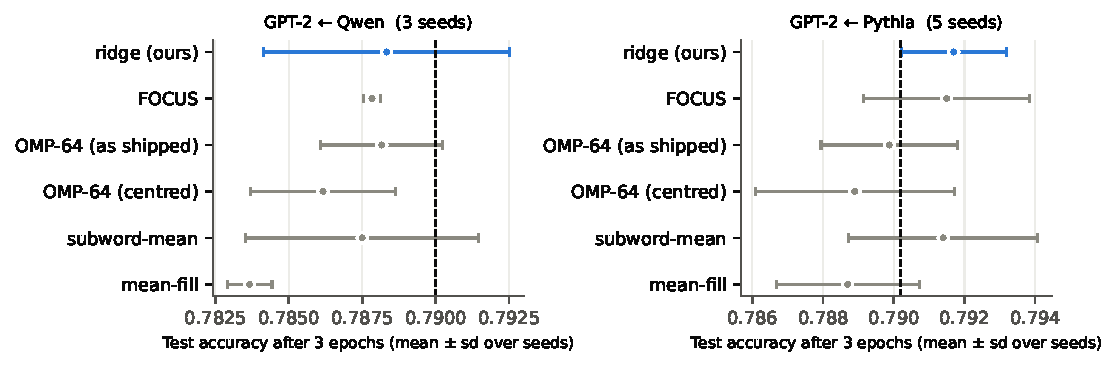
\includegraphics[width=0.95\textwidth]{figures/fig3_finetuned_accuracy.pdf}
\caption{Fine-tuned accuracy by method (mean $\pm$ sd over seeds); the dashed line is the native tokenizer.}
\label{fig:ft}
\end{figure}

\paragraph{Frozen probe} Fine-tuning can repair poor embeddings, so we also read out frozen features (Table~\ref{tab:holm}, Fig.~\ref{fig:probe}; accuracies in \ref{app:probe}). Of the 54 paired tests, 11 are significant before correction and 4 after Holm correction, all against mean fill (ridge better by $+1.4$ points on GPT-2$\leftarrow$Qwen2.5 at the middle and last layers, by $+8.3$ and $+6.7$ points on Qwen2.5$\leftarrow$GPT-2). Ridge is not significantly different from OMP-64 (centred or as shipped), FOCUS and the subword mean once corrected. The one uncorrected loss against OMP-64 centred (Qwen2.5$\leftarrow$GPT-2, last layer, $-0.65$ points, CI $-1.28$ to $-0.04$) does not survive the correction.
\begin{table}[t]
\centering\small
\caption{Frozen probe: ridge minus each method, accuracy in points (positive = ridge better). $^{*}$ 95\,\% CI excludes 0 before correction; $^{\dagger}$ still significant after Holm correction over all 54 tests.}
\label{tab:holm}
\resizebox{\textwidth}{!}{\begin{tabular}{llrrrrrr}
\toprule
Pair & Layer & OMP-64 centred & OMP-64 shipped & FOCUS & Subw.\ mean & Mean fill & Native tok. \\
\midrule
GPT-2$\leftarrow$Pythia & emb & $-$0.30 & $-$0.10 & $+$0.25 & $+$0.36 & $-$0.03 & $+$0.64 \\
 & mid & $-$0.01 & $-$0.05 & $+$0.05 & $+$0.24 & $+$0.40 & $+$0.19 \\
 & last & $-$0.24 & $-$0.06 & $+$0.58 & $+$0.22 & $+$0.26 & $+$0.11 \\
\midrule
GPT-2$\leftarrow$Qwen2.5 & emb & $+$0.32 & $+$0.21 & $-$0.25 & $-$0.04 & $+$0.21 & $+$0.68 \\
 & mid & $+$0.32 & $+$0.31 & $+$0.95$^{*}$ & $+$0.86$^{*}$ & $+$1.37$^{\dagger}$ & $+$0.09 \\
 & last & $+$0.44 & $+$0.10 & $+$0.92$^{*}$ & $+$0.83$^{*}$ & $+$1.42$^{\dagger}$ & $+$0.71 \\
\midrule
Qwen2.5$\leftarrow$GPT-2 & emb & $+$0.12 & $-$0.22 & $-$0.62$^{*}$ & $-$0.14 & $+$0.05 & $-$0.60 \\
 & mid & $-$0.16 & $-$0.34 & $+$0.75$^{*}$ & $+$0.64 & $+$8.26$^{\dagger}$ & $-$0.19 \\
 & last & $-$0.65$^{*}$ & $-$0.41 & $+$0.15 & $-$0.15 & $+$6.69$^{\dagger}$ & $-$0.61 \\
\bottomrule
\end{tabular}
}
\end{table}
\begin{figure}[t]
\centering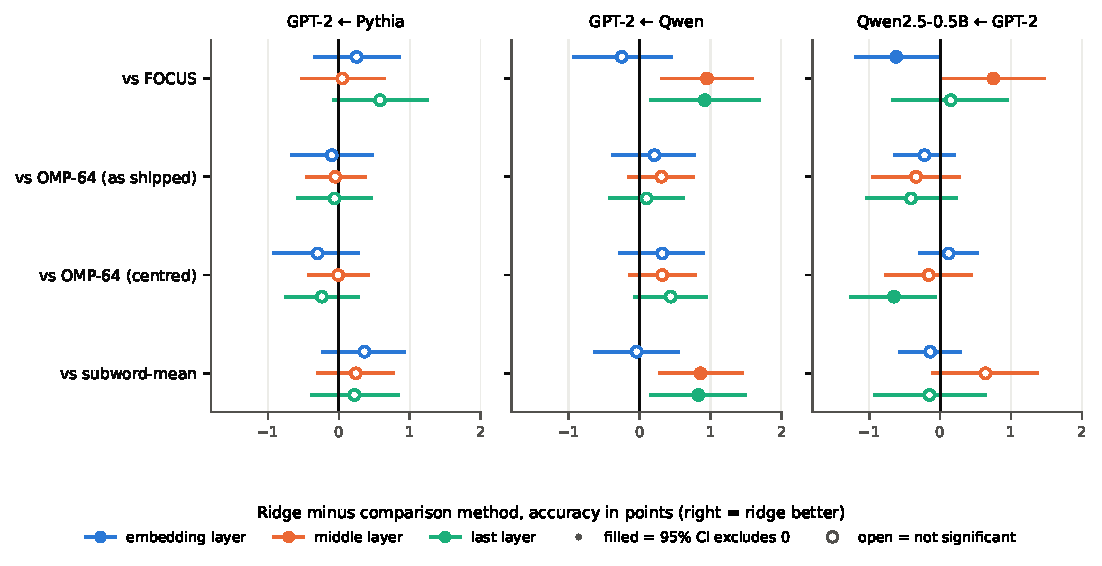
\includegraphics[width=0.95\textwidth]{figures/fig4_frozen_probe_forest.pdf}
\caption{Frozen probe: ridge minus comparison method (points; bars 95\,\% CI, uncorrected). Filled markers: interval excludes 0.}
\label{fig:probe}
\end{figure}

\paragraph{Medical abstracts} A second fine-tuning task, with another domain and label set (Table~\ref{tab:med}), asks whether the result holds beyond PubMed RCT. After three epochs all methods are within 4.7 points of each other and far above the majority rate (0.351). Ridge is comparable with the native tokenizer ($+0.0$ and $+0.1$ points) and with centred OMP-64 ($-0.2$ and $-0.0$), with every interval including 0. It is better than mean fill ($+4.4$ points, CI $+2.4$ to $+6.5$, significant after Holm correction, with the Pythia donor; $+2.5$, CI $+0.8$ to $+4.3$, with the Qwen donor, where the Holm-adjusted $p$ is 0.051) and, with the Pythia donor, than FOCUS ($+2.3$, CI $+0.5$ to $+4.2$; Holm-adjusted $p=0.11$). The comparisons with OMP-64 as shipped and the subword mean, and with FOCUS on the Qwen donor, are not significant. After the first epoch the advantage is clearer: with the Pythia donor ridge is better than FOCUS ($+3.5$ points), the subword mean ($+2.7$) and mean fill ($+4.5$), all significant after Holm correction, and with the Qwen donor it is better than mean fill ($+2.5$); it remains comparable with both OMP-64 variants. So on this task ridge is as accurate as the best baselines and clearly better than the weak ones, and we do not claim that it beats OMP-64.
\begin{table}[t]
\centering\small
\caption{Medical abstracts: test accuracy (\%) after fine-tuning the transplanted GPT-2 for 3 epochs (mean $\pm$ sd over 3 seeds) and ridge minus each method in percentage points, with the 95\,\% interval of a paired bootstrap over the 1000 test abstracts (per-abstract correctness averaged over seeds, 100\,000 resamples). $^{*}$ interval excludes 0; $^{\dagger}$ significant after Holm correction over the 10 comparisons of this epoch. The native tokenizer is a reference and is not in the correction. Majority-class accuracy is 35.1\,\%.}
\label{tab:med}
\resizebox{\textwidth}{!}{\begin{tabular}{lrrrr}
\toprule
 & \multicolumn{2}{c}{GPT-2$\leftarrow$Pythia-160m} & \multicolumn{2}{c}{GPT-2$\leftarrow$Qwen2.5-0.5B} \\
\cmidrule(lr){2-3}\cmidrule(lr){4-5}
Method & Acc.\ (\%) & Ridge minus (points) & Acc.\ (\%) & Ridge minus (points) \\
\midrule
Ridge (ours) & 60.5$\pm$0.1 & -- & 60.6$\pm$0.4 & -- \\
OMP-64 centred & 60.7$\pm$0.9 & $-$0.2\,[$-$1.3,$+$0.9] & 60.6$\pm$0.3 & $-$0.0\,[$-$1.0,$+$0.9] \\
OMP-64 as shipped & 60.7$\pm$0.6 & $-$0.2\,[$-$1.5,$+$1.0] & 59.9$\pm$0.2 & $+$0.7\,[$-$0.3,$+$1.7] \\
FOCUS & 58.1$\pm$1.0 & $+$2.3\,[$+$0.5,$+$4.2]$^{*}$ & 59.3$\pm$0.2 & $+$1.3\,[$-$0.2,$+$2.7] \\
Subword mean & 59.4$\pm$0.6 & $+$1.1\,[$-$0.5,$+$2.8] & 60.3$\pm$1.0 & $+$0.3\,[$-$0.9,$+$1.5] \\
Mean fill & 56.0$\pm$1.1 & $+$4.4\,[$+$2.3,$+$6.5]$^{*}$$^{\dagger}$ & 58.1$\pm$0.6 & $+$2.5\,[$+$0.7,$+$4.3]$^{*}$ \\
Native tokenizer & 60.4$\pm$0.6 & $+$0.0\,[$-$1.5,$+$1.5] & 60.5$\pm$0.6 & $+$0.1\,[$-$1.2,$+$1.4] \\
\bottomrule
\end{tabular}
}
\end{table}

\subsection{Ablation}
\label{sec:ablation}
We removed one component at a time and measured sentence NLL on PubMed with the GPT-2 receiver (300 and 82 new words, seed 1). Differences are against ridge fitted on all anchors (Table~\ref{tab:abl}).
\begin{table}[t]
\centering\small
\caption{Ablations (nats per sentence; positive = the ablation is worse than ridge on all anchors). $^{*}$ 95\,\% interval excludes 0. First row: full ridge against the unchanged receiver.}
\label{tab:abl}
\resizebox{\textwidth}{!}{\begin{tabular}{lrrrr}
\toprule
 & \multicolumn{2}{c}{GPT-2$\leftarrow$Pythia} & \multicolumn{2}{c}{GPT-2$\leftarrow$Qwen2.5} \\
\cmidrule(lr){2-3}\cmidrule(lr){4-5}
Variant (change from ridge fitted on all anchors) & Zero-shot & 200 steps & Zero-shot & 200 steps \\
\midrule
Full ridge vs.\ unchanged receiver (reference) & $+$2.21$^{*}$ & $+$0.49$^{*}$ & $+$0.83$^{*}$ & $-$1.00$^{*}$ \\
\midrule
Ridge on the 5000 most frequent anchors & $-$0.15$^{*}$ & $-$0.15$^{*}$ & $-$0.46$^{*}$ & $-$0.55$^{*}$ \\
No centring, calibrated length & $+$549$^{*}$ & $+$2.16$^{*}$ & $+$10.08$^{*}$ & $-$0.16 \\
No centring, raw output & $+$1678$^{*}$ & $+$2.04$^{*}$ & $+$208$^{*}$ & $-$0.63$^{*}$ \\
Own magnitude (no unit direction, no calibration) & $+$2.65$^{*}$ & $+$0.16$^{*}$ & $+$3.09$^{*}$ & $-$0.60$^{*}$ \\
Unit direction, fixed length 1.0 & $+$0.55$^{*}$ & $+$0.13$^{*}$ & $+$0.60$^{*}$ & $-$0.35$^{*}$ \\
$\lambda=10^{-4}$ & $+$0.05$^{*}$ & $-$0.02$^{*}$ & $-$0.01$^{*}$ & $+$0.00 \\
$\lambda=10^{-3}$ & $+$0.05$^{*}$ & $-$0.02$^{*}$ & $+$0.00 & $+$0.00 \\
$\lambda=10^{-2}$ & $+$0.04$^{*}$ & $-$0.01$^{*}$ & $+$0.06$^{*}$ & $-$0.00 \\
$\lambda=0.1$ & $+$0.00 & $+$0.00 & $+$0.17$^{*}$ & $-$0.01 \\
$\lambda=1$ & $+$0.24$^{*}$ & $+$0.07$^{*}$ & $+$1.79$^{*}$ & $-$0.34$^{*}$ \\
Mean of word pieces (calibrated) & $+$8.76$^{*}$ & $+$2.87$^{*}$ & $+$4.78$^{*}$ & $+$0.47$^{*}$ \\
\bottomrule
\end{tabular}
}
\end{table}
\textbf{Centring} is essential zero-shot: without it the NLL rises by 549 nats with Pythia and 10 with Qwen2.5; after training the new rows the loss is 2.2 nats with Pythia, and with Qwen2.5 the uncentred variants are level or slightly better. \textbf{Length calibration} helps zero-shot (no scale at all: $+2.7$ to $+3.1$ nats; a fixed length of 1: $+0.6$), but after training the uncalibrated variants are 0.35 to 0.6 nats better with Qwen2.5 and 0.13 to 0.16 worse with Pythia, so its benefit is a zero-shot benefit. \textbf{The regularisation strength} is not critical: between $10^{-4}$ and $10^{-2}$ the NLL changes by at most 0.06 nats ($\lambda=0.1$ costs 0.17 with Qwen2.5, $\lambda=1$ is clearly too large zero-shot). \textbf{The ridge direction} is far better than the mean of word pieces ($+8.8$ and $+4.8$ nats zero-shot). Fitting on the 5000 most frequent anchors is better than on all anchors ($-0.15$ and $-0.46$ zero-shot), which supports selecting by the training objective. These ablations use one seed, one text domain and two pairs, and the word sets of an earlier selection rule that also required occurrences in the evaluation text (the rule of Section~\ref{par:rvprotocol} uses the training text only); all variants in the table share the same words.

\subsection{Control: the penalty or the anchors?}
\label{sec:control}
Ridge fitted on the 5000 most frequent anchors differs from our earlier least-squares baseline in two ways, the penalty and the anchor subset. To separate them we added plain least squares fitted on the same 5000 anchors (PubMed, seed 0, the four small pairs, the same words as the 17-run set; the conditions shared with those runs reproduce them exactly). With the same anchors the two maps are close (Table~\ref{tab:control}, first column): the difference lies between $-0.14$ and $+0.17$ nats, ridge is better in three of the eight comparisons, worse in three and level in two, and five of the six significant differences survive Holm correction over the eight. Least squares on the frequent anchors is better than least squares on all anchors in six of eight comparisons (by 0.06 to 0.54 nats) and never worse (second column). Ridge and least squares on all anchors are also close (third column, $-0.06$ to $+0.02$ nats). With tens of thousands of anchors, the gain over our least-squares baseline therefore comes from fitting on the frequent anchors, together with the calibrated length that all variants share, and not from the penalty; the penalty matters when anchors are scarce (Section~\ref{sec:scarce}). We keep the name ``ridge'' because it is the variant that remains stable in both regimes, and we do not claim that the penalty explains the gains in the main tables.
\begin{table}[t]
\centering\small
\caption{Control for the ridge penalty (nats per sentence; negative = the first method is better). $^{*}$ the 95\,\% abstract-level bootstrap interval excludes 0; $^{\dagger}$ significant after Holm correction over the eight comparisons of the column. ``LS'' is plain least squares (minimum-norm), all maps with the calibrated length.}
\label{tab:control}
\resizebox{\textwidth}{!}{\begin{tabular}{llccc}
\toprule
Pair & Steps & ridge[freq5000] $-$ LS[freq5000] & LS[freq5000] $-$ LS (all anchors) & ridge[all] $-$ LS (all anchors) \\
\midrule
GPT-2 $\leftarrow$ Pythia-160m & 0 & $+$0.17\,[$+$0.07,$+$0.28]$^{*}$$^{\dagger}$ & $-$0.36\,[$-$0.47,$-$0.25]$^{*}$$^{\dagger}$ & $-$0.04\,[$-$0.06,$-$0.02]$^{*}$$^{\dagger}$ \\
 & 200 & $+$0.12\,[$+$0.05,$+$0.18]$^{*}$$^{\dagger}$ & $-$0.22\,[$-$0.30,$-$0.14]$^{*}$$^{\dagger}$ & $+$0.02\,[$+$0.01,$+$0.03]$^{*}$$^{\dagger}$ \\
\addlinespace
GPT-2 $\leftarrow$ Qwen2.5-0.5B & 0 & $-$0.13\,[$-$0.21,$-$0.04]$^{*}$$^{\dagger}$ & $-$0.47\,[$-$0.62,$-$0.33]$^{*}$$^{\dagger}$ & $+$0.02\,[$+$0.01,$+$0.03]$^{*}$$^{\dagger}$ \\
 & 200 & $+$0.01\,[$-$0.02,$+$0.03] & $-$0.54\,[$-$0.62,$-$0.45]$^{*}$$^{\dagger}$ & $+$0.00\,[$-$0.00,$+$0.00] \\
\addlinespace
OPT-125m $\leftarrow$ Pythia-160m & 0 & $+$0.12\,[$+$0.01,$+$0.23]$^{*}$ & $-$0.10\,[$-$0.22,$+$0.02] & $-$0.01\,[$-$0.03,$+$0.01] \\
 & 200 & $+$0.10\,[$-$0.00,$+$0.20] & $-$0.06\,[$-$0.17,$+$0.04] & $-$0.06\,[$-$0.10,$-$0.02]$^{*}$$^{\dagger}$ \\
\addlinespace
OPT-125m $\leftarrow$ Qwen2.5-0.5B & 0 & $-$0.14\,[$-$0.22,$-$0.08]$^{*}$$^{\dagger}$ & $-$0.21\,[$-$0.36,$-$0.06]$^{*}$$^{\dagger}$ & $+$0.01\,[$+$0.01,$+$0.02]$^{*}$$^{\dagger}$ \\
 & 200 & $-$0.07\,[$-$0.11,$-$0.03]$^{*}$$^{\dagger}$ & $-$0.25\,[$-$0.34,$-$0.16]$^{*}$$^{\dagger}$ & $-$0.01\,[$-$0.02,$+$0.00] \\
\bottomrule
\end{tabular}
}
\end{table}
\begin{figure}[t]
\centering
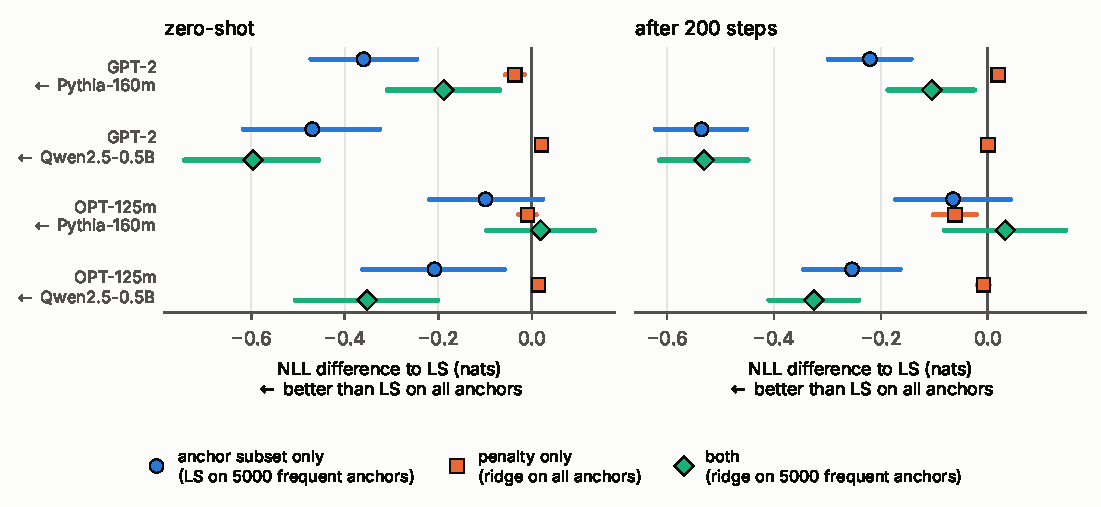
\includegraphics[width=\textwidth]{figures/fig_ls_decomp}
\caption{What separates ridge from least squares: NLL difference to least squares on all anchors (all with the calibrated length; PubMed seed 0; 95\,\% abstract-level bootstrap intervals). The anchor subset alone (blue) gives most of the gain; the penalty alone (orange) changes little; both together (green) are not consistently better than the subset alone. The same numbers are in Table~\ref{tab:control}.}
\label{fig:lsdecomp}
\end{figure}

\subsection{Scarce anchors: why regularise}
\label{sec:scarce}
With tens of thousands of anchors, a well-conditioned least-squares fit needs little regularisation. It should matter when the number of anchors $n$ is small or close to the embedding dimension $d$, where the least-squares problem is ill-conditioned: for $n<d$ it is underdetermined (we use the minimum-norm solution), and the error of minimum-norm least squares is known to peak near $n=d$ \cite{hastie2022surprises}. We tested this on the two GPT-2 pairs of the real vocabulary setting (PubMed, seed 1, zero-shot) by fitting both maps on $n=d/2$, $d$ and $2d$ anchors drawn uniformly at random without replacement from all whole-word anchors (five independent random subsets per $n$, not frequency-selected) and on all anchors, with the same calibrated length for both. Fig.~\ref{fig:cos} shows the held-out cosine between predicted and true receiver rows, measured on 2000 anchors not used for fitting and averaged over five random subsets per $n$, for $n/d$ from 0.1 to about 30; Table~\ref{tab:anchors} gives the NLL.
\begin{figure}[t]
\centering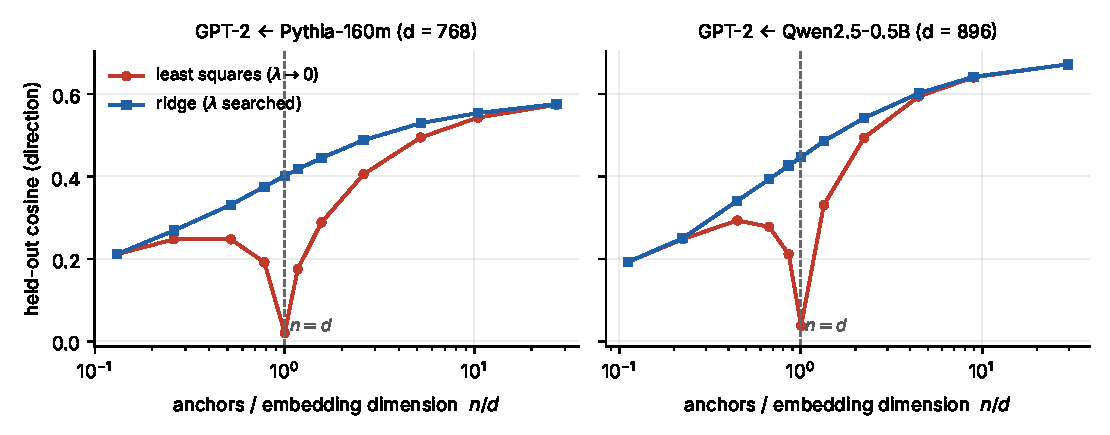
\includegraphics[width=0.97\textwidth]{figures/fig_ls_vs_ridge_cosine.pdf}
\caption{Held-out cosine between predicted and true receiver embeddings against the number of anchors relative to the donor dimension, for plain least squares (minimum-norm solution) and ridge ($\lambda$ searched on held-out anchors). The dashed line marks $n=d$.}
\label{fig:cos}
\end{figure}
\begin{table}[t]
\centering\small
\caption{Plain least squares (LS) against ridge when only $n$ anchors are used to fit the map (PubMed, seed 1, zero-shot; NLL in nats per sentence; mean over five random anchor subsets per $n$, one for all anchors). The difference column gives the mean and the minimum and maximum over the subsets. Both maps use the same calibrated length. The unchanged receiver has an NLL of 142.3 (Pythia donor) and 147.3 (Qwen donor).}
\label{tab:anchors}
\resizebox{\textwidth}{!}{\begin{tabular}{llrrr}
\toprule
Pair & $n$ ($n/d$) & LS & Ridge & Ridge $-$ LS: mean [min, max over subsets] \\
\midrule
GPT-2$\leftarrow$Pythia-160m & 384 (0.5) & 203.6 & 147.6 & $-$55.99 [$-$100.45, $-$12.92] \\
 & 768 (1.0) & 275.4 & 146.5 & $-$128.95 [$-$519.01, $-$13.93] \\
 & 1,536 (2.0) & 147.3 & 145.5 & $-$1.74 [$-$1.96, $-$1.63] \\
 & 22,781 (29.7) & 144.5 & 144.5 & $-$0.05 (one subset) \\
\midrule
GPT-2$\leftarrow$Qwen2.5-0.5B & 448 (0.5) & 358.1 & 153.5 & $-$204.57 [$-$733.99, $-$7.73] \\
 & 896 (1.0) & 249.9 & 152.9 & $-$97.02 [$-$180.47, $-$18.94] \\
 & 1,792 (2.0) & 149.9 & 150.7 & $+$0.85 [$+$0.72, $+$1.12] \\
 & 28,512 (31.8) & 148.1 & 148.1 & $+$0.01 (one subset) \\
\bottomrule
\end{tabular}
}
\end{table}
Least squares collapses when $n$ is near $d$: its held-out cosine falls to 0.02 at $n=768$ (Pythia donor) and 0.04 at $n=900$ (Qwen donor), while ridge stays at about 0.40 and 0.45, and below $n=d$ least squares is already worse than ridge. The NLL shows the same pattern (Table~\ref{tab:anchors}). Ridge is better in every one of the five subsets at $n=d/2$ (by 13 to 100 nats with the Pythia donor and 8 to 734 with the Qwen donor) and at $n=d$ (by 14 to 519 and 19 to 180 nats); the size of the gap varies a lot between subsets, because the minimum-norm least-squares fit occasionally fails badly near $n=d$, so the means are dominated by those cases and the ranges should be read with them. At $n=2d$ the picture is mixed and consistent across subsets: ridge is 1.6 to 2.0 nats better in all five with the Pythia donor but 0.7 to 1.1 nats \emph{worse} in all five with the Qwen donor. With all anchors ($n/d\approx30$) the two do not differ significantly (differences of $-0.05$ and $+0.01$ nats). Regularisation therefore matters in the scarce-anchor regime, roughly $n\lesssim 2d$, and not when there are tens of thousands of anchors as in our main experiments. This regime arises when two tokenizers share few whole-word tokens, for example with a small donor vocabulary or a restricted anchor list; the pairs we tested do not have this property, so these are controlled subsamples, not a test on such pairs. Like the ablation, this test used the word sets of the earlier selection rule; both maps in it share the same words.

\paragraph{Choice of $\lambda$ in the scarce regime} $\lambda$ was chosen as in the main method, by cosine on held-out anchors (10\,\% of the anchors, at least 50, at most 20\,\%; about 50 anchors at $n=d/2$). It was the largest value of the grid ($\lambda=1$) in all five subsets at $n\le2d$ for both donors, which raises the question whether the grid is too narrow. We therefore repeated the selection with a grid extended to $\lambda=1000$. It then chose $\lambda=10$ at $n\le d$ for the Pythia donor and for $n=d/2$ with the Qwen donor, but the NLL did not improve: it was 0.03 to 0.5 nats higher with the Pythia donor and 2.6 nats higher at $n=d/2$ with the Qwen donor, and identical at the other sizes. The grid edge therefore does not limit the result: selecting $\lambda$ by cosine and measuring NLL agree on $\lambda\approx1$ to 10 here. The results rest on two pairs, one seed and five random subsets per $n$.

\subsection{Mapping time}
\label{sec:speed}
An earlier timing from our experiment logs compared OMP on a GPU with ridge on a CPU and is not used. We therefore timed both on the \emph{same device and dtype}: float32, the official \texttt{batch\_omp} and our torch implementation of Eq.~\eqref{eq:ridge}, GPT-2 and Pythia-160m or Qwen2.5-0.5B embedding matrices (42\,257 anchors), $K$ donor-only tokens, after a warm-up with device synchronisation, median of 5 repeats, on 2 CPU threads and one Tesla T4 GPU. ``Fixed'' uses one solve with $\lambda=0.01$, supported by the ablation; ``search'' is the procedure of Section~\ref{sec:method} (five validation solves and one final solve).
\begin{table}[t]
\centering\small
\caption{Time to build the new rows (seconds, median of 5, float32). Ratio = OMP-64 time divided by fixed-$\lambda$ ridge time. The length calibration is not included.}
\label{tab:speed}
\resizebox{\textwidth}{!}{\begin{tabular}{lrrrrrrrrr}
\toprule
 & & \multicolumn{4}{c}{CPU (2 threads), s} & \multicolumn{4}{c}{GPU (Tesla T4), s} \\
\cmidrule(lr){3-6}\cmidrule(lr){7-10}
Pair & $K$ & OMP-64 & Ridge fixed & Ridge search & Ratio & OMP-64 & Ridge fixed & Ridge search & Ratio \\
\midrule
GPT-2 $\leftarrow$ Pythia & 82 & 2.59 & 0.547 & 2.85 & 5$\times$ & 0.16 & 0.043 & 0.12 & 4$\times$ \\
 & 300 & 9.95 & 0.551 & 2.93 & 18$\times$ & 0.47 & 0.043 & 0.14 & 11$\times$ \\
 & 1000 & 30.28 & 0.572 & 2.93 & 53$\times$ & 1.58 & 0.043 & 0.14 & 37$\times$ \\
 & 3000 & 87.62 & 0.573 & 2.96 & 153$\times$ & 5.11 & 0.039 & 0.14 & 131$\times$ \\
\midrule
GPT-2 $\leftarrow$ Qwen2.5 & 82 & 3.71 & 0.757 & 4.00 & 5$\times$ & 0.24 & 0.058 & 0.21 & 4$\times$ \\
 & 300 & 12.66 & 0.766 & 4.01 & 17$\times$ & 0.68 & 0.037 & 0.21 & 18$\times$ \\
 & 1000 & 37.98 & 0.758 & 3.96 & 50$\times$ & 1.78 & 0.039 & 0.21 & 46$\times$ \\
 & 3000 & 109.74 & 0.784 & 4.08 & 140$\times$ & 5.61 & 0.039 & 0.21 & 144$\times$ \\
\bottomrule
\end{tabular}
}
\end{table}
\begin{figure}[t]
\centering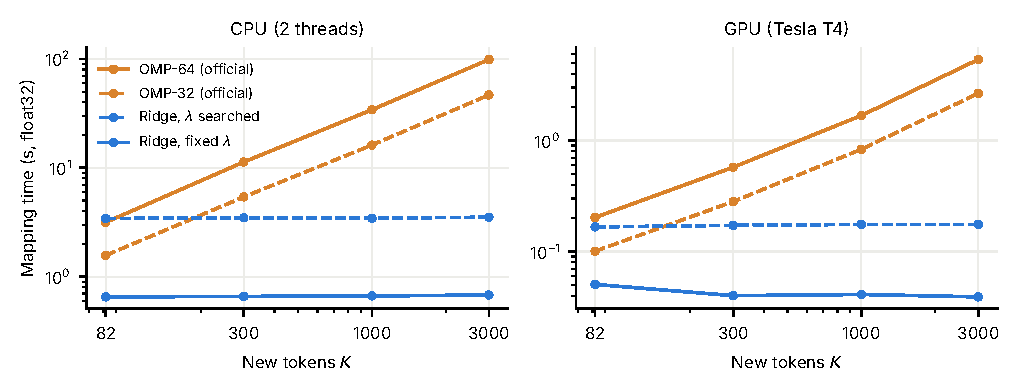
\includegraphics[width=0.95\textwidth]{figures/fig_speed.pdf}
\caption{Mapping time against the number of new tokens $K$ (mean of the two pairs, float32, log--log scale).}
\label{fig:speed}
\end{figure}
With a fixed $\lambda$, ridge is faster than official OMP-64 in every setting: 4 to 5 times at $K=82$, 11 to 18 times at 300, 37 to 53 times at 1000 and 131 to 153 times at 3000 (Table~\ref{tab:speed}). Ridge time is almost independent of $K$, whereas OMP grows linearly with it (about 29 to 45\,ms per token on the CPU and 1.6 to 3\,ms per token on the T4). With the $\lambda$ search, ridge is level with OMP at $K=82$ (0.9 to 1.3 times) and 3 to 3.5, 8.5 to 11 and 27 to 36 times faster at 300, 1000 and 3000. One caution applies: the speed advantage concerns the mapping step only. The reported NLL results use a float64 ridge, so we checked that the float32 solve used in the timing gives the same directions: for 3000 new tokens, the cosine between the float32 and float64 directions is at least 0.999999 for every token (minimum and mean both 1.000000 at six decimals) for GPT-2$\leftarrow$Pythia-160m (36\,938 anchors) and GPT-2$\leftarrow$Qwen2.5-0.5B (42\,257 anchors).

\section{Discussion}
\label{sec:discussion}
\paragraph{What the evidence supports} Ridge is a simple, gradient-free initialiser that is better than the strongest official baseline (centred OMP-64) in real vocabulary expansion with small receivers, measured by NLL on sentences that contain the new words: in 23 of 24 comparisons, by 1.3 to 3.2 nats zero-shot and by less after training. Against seven baselines on seven pairs up to 1.5B parameters it is significantly better in 78 of 98 comparisons (74 after Holm correction) and significantly worse in one, and it is better than learned initialisers (official token distillation and our own version) in 39 of 40 comparisons without using any training text for the map. After fine-tuning it is as accurate as the native tokenizer and the best baselines on two classification tasks, and clearly better than mean fill. The ablations indicate why: the receiver and donor spaces share a large common component that must be removed before a linear map can be fitted, and a regression that sees all anchors at once gives better directions than a sparse reconstruction of 64 of them, even when both use the same length rule (Table~\ref{tab:rv}). The regularisation in ridge matters mainly when anchors are scarce: with $n\lesssim 2d$ anchors, plain least squares is much worse in NLL, and with tens of thousands of anchors the two are close (Section~\ref{sec:scarce}); the zero-shot advantage over least squares in all seven pairs then comes mainly from fitting on the most frequent anchors; with least squares fitted on the same anchors, the two differ by at most 0.17 nats and neither is consistently better (Section~\ref{sec:control}). The same pattern appears on arXiv abstracts, where ridge is significantly better in 49 of 56 comparisons with the baselines (Section~\ref{sec:arxiv}).

\paragraph{Scope} The results concern small receivers (125M to 1.5B parameters, plus one 7B receiver tested zero-shot), English text, two text domains (PubMed, and arXiv for four pairs on one seed) and NLL on sentences that contain the new words. At 1B parameters and above no initialisation, ridge included, beat leaving the words split (the 7B receiver tested zero-shot behaves the same), so the benefit shown there is a shorter input. The margins over centred OMP-64 are small after training, and ridge is not better than every baseline in every comparison: Procrustes is better zero-shot on OPT-125m$\leftarrow$Pythia-160m (on arXiv as well, and there least squares is better too), and on the two largest receivers many comparisons are not significant. After fine-tuning, strong initialisations perform alike. The speed advantage concerns the mapping step on a given device; the total initialisation time, which includes the NLL calibration, is dominated by forward passes and is of the same order as that of the official token distillation.

\paragraph{Limitations} Downstream evidence is two classification tasks, and real vocabulary expansion is measured by NLL, not by a task. The receivers are small to medium (125M to 1.5B parameters), and a 7B receiver was tested zero-shot only. Only one receiver is untied (Pythia-1B), its output rows were built from the donor output embeddings, a design choice we did not vary, and it has 52 new words and 89 test sentences. GPT-2 large and Pythia-1B have two seeds and Qwen2.5-1.5B one, and the tables use seed 1. The text domains are PubMed (all runs) and arXiv (four small pairs, one seed). The seeds resample sentences and training batches, not words or abstracts, so they measure training and sampling noise. The ablations and the scarce-anchor test use one seed, one text domain and the word sets of an earlier selection rule that also used evaluation-text occurrences (shared by all methods within each table). Multiplicity is corrected for the frozen probe, the 24-, 98- and 168-comparison families, the learned-baseline family and the medical-abstracts task, not for the other tables. The bootstrap resamples abstracts but not new words. We tested a receiver of 3B parameters or more only zero-shot (Qwen2.5-7B, one pair, one seed, float16) and no multilingual or non-Latin-script pair, so the claims are confined to small receivers, English text and NLL. The length $c$ is a single scalar for all new tokens; a per-token or frequency-dependent length was not tested. Learned initialisers are represented by the official AweDist on four small pairs and GPT-2 large, with a larger text budget than ridge uses and its defaults except the number of snippets (5 instead of 25, see Section~\ref{sec:learned}), and by our own TokDist; AweDist failed on Qwen2.5-1.5B and was not run on the untied Pythia-1B, and ZeTT and TokAlign were not run, so how far a closed-form initialisation is from a fully trained one remains open beyond these cases. SALT is represented only by our simplified adaptation, and LS, Procrustes and OMP-32 are also our own implementations. WECHSEL was run on the PubMed seed-1 runs only, in same-language mode. The medical-abstracts task has 1000 test abstracts, so accuracy differences of 1 to 2 points are not resolved.

\section{Conclusion}
\label{sec:conclusion}
A closed-form ridge map from donor to receiver embeddings, fitted on centred anchors and scaled by a single calibrated length, is a competitive way to initialise new tokens for small receivers (125M to 1.5B parameters), judged by NLL on sentences that contain the new words. In 12 real vocabulary-expansion runs it was better than the official OMP-64 in 23 of 24 comparisons, by small margins, and its mapping step is much cheaper than OMP as the number of new tokens grows. On seven pairs up to 1.5B parameters it was significantly better than seven baselines in 78 of 98 comparisons, and it was better than learned initialisers in 39 of 40, but for the receivers of 1B parameters or more (including a 7B receiver tested zero-shot) no initialisation, ridge included, beat leaving the words split. We also showed that the official OMP needs centred inputs on GPT-2 receivers, that after fine-tuning on two classification tasks ridge matches the native tokenizer and the best baselines, and that the penalty matters only when anchors are scarce ($n\lesssim2d$), whereas with many anchors the gain comes from fitting on the most frequent ones; the pattern holds on a second domain (arXiv). The added tokens shorten the sentences that contain them by 3 to 6\,\%, a property of the vocabulary and not of the initialiser. Larger models, more text domains and more seeds at that scale, more downstream tasks and further learned initialisers are the natural next comparisons.

\section*{Declaration of competing interest}
The authors declare that they have no known competing financial interests or personal relationships that could have appeared to influence the work reported in this paper.

\section*{CRediT authorship contribution statement}
\textbf{Shibdas Bhattacharya:} Conceptualization, Methodology, Software, Investigation, Formal analysis, Writing -- original draft. \textbf{Haider Banka:} Supervision, Writing -- review \& editing.

\section*{Funding}
This research did not receive any specific grant from funding agencies in the public, commercial, or not-for-profit sectors.

\section*{Data and code availability}
All data are public (PubMedQA, PubMed 20k RCT, medical abstracts, WikiText-2, arXiv abstracts; the exact arXiv set we used is in the repository) and all models are public. The code, notebooks, result files, analysis scripts, a requirements file, a script that records the environment and a reproducibility guide are publicly available at \url{https://github.com/shib1989/calibrated-ridge-transplant} (DOI: \href{https://doi.org/10.5281/zenodo.24058629}{10.5281/zenodo.24058629}). The guide maps every table and figure to a notebook and a script. \ref{app:repro} lists checkpoints, data, hyperparameters and seeds. The experiment notebooks install packages without version pins; the notebooks of the real-vocabulary runs record the environment of their session (\texttt{environment.json}), and for the earlier experiments the repository records the environment afterwards and gives a rerun check.

\section*{Declaration of generative AI use in the writing process}
During the preparation of this work the authors used Claude (Anthropic) to help write and debug code for the experiments and statistical analysis, to generate tables and figures from the results, and to draft and edit the text. After using this tool, the authors reviewed and edited the content and take full responsibility for the content of the publication.

\appendix
\section{Real vocabulary expansion: all runs}
\label{app:rv}
\begin{table}[H]
\centering\scriptsize
\caption{Ridge minus each method, NLL per sentence in nats, for each of the 12 runs (negative = ridge better; $^{*}$ 95\,\% interval excludes 0). ``vs.\ unch.'' = ridge minus the unchanged receiver; OMP-64c = official OMP-64 on centred inputs; OMP-64s = as shipped; OMP-32 = our scikit-learn implementation.}
\label{tab:rvfull}
\resizebox{\textwidth}{!}{\begin{tabular}{lrrrrrrrrrr}
\toprule
 & & & \multicolumn{4}{c}{Zero-shot} & \multicolumn{4}{c}{After 200 steps} \\
\cmidrule(lr){4-7}\cmidrule(lr){8-11}
Receiver$\leftarrow$donor & Seed & Words & vs.\ unch. & $-$OMP-64c & $-$OMP-64s & $-$OMP-32 & vs.\ unch. & $-$OMP-64c & $-$OMP-64s & $-$OMP-32 \\
\midrule
GPT-2$\leftarrow$Pythia & 0 & 300 & $+$2.54$^{*}$ & $-$1.55$^{*}$ & $-$3526$^{*}$ & $-$0.58$^{*}$ & $+$0.42$^{*}$ & $-$0.62$^{*}$ & $-$96.6$^{*}$ & $-$0.44$^{*}$ \\
GPT-2$\leftarrow$Pythia & 1 & 300 & $+$2.32$^{*}$ & $-$1.68$^{*}$ & $-$3179$^{*}$ & $-$0.70$^{*}$ & $+$0.21 & $-$0.52$^{*}$ & $-$76.5$^{*}$ & $-$0.51$^{*}$ \\
GPT-2$\leftarrow$Pythia & 2 & 300 & $+$2.29$^{*}$ & $-$1.77$^{*}$ & $-$3194$^{*}$ & $-$0.71$^{*}$ & $-$0.03 & $-$0.65$^{*}$ & $-$75.7$^{*}$ & $-$0.64$^{*}$ \\
GPT-2$\leftarrow$Qwen2.5 & 0 & 126 & $+$0.56$^{*}$ & $-$3.23$^{*}$ & $-$458$^{*}$ & $-$1.18$^{*}$ & $-$1.13$^{*}$ & $-$0.19$^{*}$ & $-$0.64$^{*}$ & $-$0.44$^{*}$ \\
GPT-2$\leftarrow$Qwen2.5 & 1 & 126 & $+$0.34$^{*}$ & $-$3.23$^{*}$ & $-$467$^{*}$ & $-$1.20$^{*}$ & $-$1.41$^{*}$ & $-$0.17$^{*}$ & $-$0.52$^{*}$ & $-$0.56$^{*}$ \\
GPT-2$\leftarrow$Qwen2.5 & 2 & 126 & $+$0.39$^{*}$ & $-$3.14$^{*}$ & $-$477$^{*}$ & $-$1.15$^{*}$ & $-$1.18$^{*}$ & $-$0.05 & $-$0.60$^{*}$ & $-$0.50$^{*}$ \\
OPT-125m$\leftarrow$Pythia & 0 & 300 & $+$1.29$^{*}$ & $-$1.25$^{*}$ & $-$1.02$^{*}$ & $-$0.27$^{*}$ & $-$0.86$^{*}$ & $-$0.67$^{*}$ & $-$0.63$^{*}$ & $-$0.19 \\
OPT-125m$\leftarrow$Pythia & 1 & 300 & $+$1.15$^{*}$ & $-$1.48$^{*}$ & $-$1.04$^{*}$ & $-$0.39$^{*}$ & $-$1.43$^{*}$ & $-$0.75$^{*}$ & $-$0.72$^{*}$ & $-$0.42$^{*}$ \\
OPT-125m$\leftarrow$Pythia & 2 & 300 & $+$1.23$^{*}$ & $-$1.45$^{*}$ & $-$1.20$^{*}$ & $-$0.23$^{*}$ & $-$1.15$^{*}$ & $-$0.84$^{*}$ & $-$0.81$^{*}$ & $-$0.41$^{*}$ \\
OPT-125m$\leftarrow$Qwen2.5 & 0 & 126 & $+$0.03 & $-$2.52$^{*}$ & $-$2.41$^{*}$ & $-$1.08$^{*}$ & $-$2.57$^{*}$ & $-$0.60$^{*}$ & $-$0.59$^{*}$ & $-$0.42$^{*}$ \\
OPT-125m$\leftarrow$Qwen2.5 & 1 & 126 & $-$0.20 & $-$2.50$^{*}$ & $-$2.39$^{*}$ & $-$1.16$^{*}$ & $-$2.83$^{*}$ & $-$0.40$^{*}$ & $-$0.49$^{*}$ & $-$0.44$^{*}$ \\
OPT-125m$\leftarrow$Qwen2.5 & 2 & 126 & $-$0.06 & $-$2.52$^{*}$ & $-$2.48$^{*}$ & $-$1.11$^{*}$ & $-$2.55$^{*}$ & $-$0.46$^{*}$ & $-$0.48$^{*}$ & $-$0.45$^{*}$ \\
\bottomrule
\end{tabular}
}
\end{table}

\section{Frozen probe: accuracies}
\label{app:probe}
\begin{table}[H]
\centering\small
\caption{Frozen-probe accuracy (logistic regression on frozen features; emb = embedding layer, mid = middle layer, last = last layer). Majority-class accuracy 0.334.}
\label{tab:frozenacc}
\resizebox{\textwidth}{!}{\begin{tabular}{lrrrrrrrrr}
\toprule
 & \multicolumn{3}{c}{GPT-2$\leftarrow$Pythia} & \multicolumn{3}{c}{GPT-2$\leftarrow$Qwen2.5} & \multicolumn{3}{c}{Qwen2.5$\leftarrow$GPT-2} \\
\cmidrule(lr){2-4}\cmidrule(lr){5-7}\cmidrule(lr){8-10}
Method & emb & mid & last & emb & mid & last & emb & mid & last \\
\midrule
\textbf{Ridge, calibrated (ours)} & 0.670 & 0.763 & 0.736 & 0.670 & 0.762 & 0.742 & 0.674 & 0.790 & 0.743 \\
FOCUS & 0.667 & 0.762 & 0.730 & 0.673 & 0.751 & 0.733 & 0.680 & 0.782 & 0.742 \\
OMP-64, as shipped & 0.670 & 0.763 & 0.737 & 0.668 & 0.758 & 0.741 & 0.676 & 0.793 & 0.747 \\
OMP-64, centred inputs & 0.673 & 0.763 & 0.739 & 0.667 & 0.758 & 0.738 & 0.673 & 0.791 & 0.750 \\
Subword mean & 0.666 & 0.760 & 0.734 & 0.670 & 0.753 & 0.734 & 0.676 & 0.783 & 0.745 \\
Mean fill & 0.670 & 0.759 & 0.734 & 0.668 & 0.748 & 0.728 & 0.674 & 0.707 & 0.676 \\
Native tokenizer (reference) & 0.663 & 0.761 & 0.735 & 0.663 & 0.761 & 0.735 & 0.680 & 0.791 & 0.749 \\
\bottomrule
\end{tabular}
}
\end{table}

\section{Reproducibility details}
\label{app:repro}
\paragraph{Checkpoints and data}\sloppy Receivers: \texttt{openai-community/gpt2}, \texttt{gpt2-medium} and \texttt{gpt2-large}, \texttt{facebook/opt-125m}, \texttt{EleutherAI/pythia-1b}, \texttt{Qwen/Qwen2.5-0.5B}, \texttt{Qwen2.5-1.5B} and \texttt{Qwen2.5-7B}. Donors: \texttt{EleutherAI/pythia-160m} and \texttt{pythia-410m}, \texttt{Qwen/Qwen2.5-0.5B}, \texttt{openai-community/gpt2}. All are loaded from the \texttt{main} branch in float32 (the 7B receiver in float16, split over two GPUs); the revision hashes are in the repository (\texttt{environment.json}). Domain text: the first 4000 abstracts of \texttt{qiaojin/PubMedQA} (configuration \texttt{pqa\_artificial}, streamed). General text: the first 30\,000 lines of \texttt{Salesforce/wikitext} (\texttt{wikitext-2-raw-v1}, training split, headings removed). arXiv: abstracts retrieved through the arXiv API (500 requested from each of cs.LG, cs.CV, cs.CL, stat.ML, math.PR, math.OC, physics.optics and cond-mat.mtrl-sci, at least 600 characters, shuffled with seed 0; 3621 abstracts, stored in the repository). Downstream: PubMed 20k RCT.

\paragraph{Reference environment} Recorded by the notebook of the v6 runs, in a cloud notebook session with Tesla T4 GPUs (15\,GB each; the runs use one), driver 580.178.04, CUDA 13.0 and cuDNN 9.27: Python 3.13.16, PyTorch 2.11.0, Transformers 5.20.2, NumPy 2.1.3, SciPy 1.16.3, scikit-learn 1.6.1, datasets 4.8.5, mergekit 0.1.5, \texttt{wechsel} 0.0.4 and \texttt{deepfocus} 1.0.1. The v6 and v9 notebooks record their own environment in the session of the runs (\texttt{environment.json}: package versions, the checkpoint revisions actually loaded, the hash of the fastText file). For the earlier experiments (tokenizer swap, fine-tuning, frozen probe, ablations, anchors, timing) the versions at the time of the runs were not recorded; the repository lists the hub revisions at capture and the dataset revisions (PubMedQA, WikiText, PubMed 20k RCT).

\paragraph{Preprocessing} Text is whitespace-normalised and split into sentences after ``.'', ``!'' or ``?'' followed by white space; sentences of 8 to 60 words are kept. Abstracts are split 70/30 by position. Text is segmented into runs of letters, runs of digits, runs of underscores, runs of other symbols and white space, each with an optional leading space (the regular expression is in \texttt{REPRODUCE.md}). Calibration uses 300 sentences with new words and 150 without (half domain text, half the first half of WikiText); evaluation uses up to 600 sentences with new words and 200 sentences for each control set (the second half of WikiText for the general control). If fewer sentences exist, all are used: for Pythia-1B the 89 evaluation sentences are the same for every seed.

\paragraph{Hyperparameters} Ridge: $\lambda\in\{10^{-4},\dots,1\}$ relative to the mean diagonal of $\tilde X^\top\tilde X$, chosen by held-out cosine (10\,\% of the fitting anchors, at least 50, at most 20\,\%), then refitted; anchor subsets all and 5000 most frequent; length grid $c\in\{0.3,0.5,0.6,0.7,0.8,0.9,1,1.2,1.5\}$. OMP-64: official \texttt{batch\_omp} (mergekit 0.1.5), $k=64$. OMP-32: scikit-learn \texttt{orthogonal\_mp} on unit-normalised centred vectors. SALT-ours: 2000 nearest anchors by cosine, ridge with intercept, relative $\lambda=10^{-2}$. WECHSEL: package version 0.0.4, same-language mode, \texttt{cc.en.300.bin}, 10 neighbours, temperature 0.1. Training of new rows: 200 steps, AdamW, learning rate $10^{-3}$, weight decay 0, batches of 8 sentences with new words from a pool of at most 2000, receiver in evaluation mode, old rows restored exactly; for Qwen2.5-1.5B micro-batches of 2 with the loss divided by the tokens of the whole batch. Maps use float64 except official OMP (float32 on the GPU).

\paragraph{Abstract identifiers} The result files do not store the abstract of each evaluation sentence. We recovered them by rebuilding the sentence sampling (same 4000 PubMedQA abstracts, 70/30 split by abstract, seed, and order of the random draws) with the stored word list, and accepted a run only if the rebuilt token counts of the evaluation sentences equalled the stored counts for both the split and the new vocabulary; all 17 runs passed. The notebook is \texttt{recover\_abstract\_ids\_v6.ipynb} and the identifiers are in \texttt{results/abstract\_ids/}. The learned-baseline runs use the same evaluation sentences as the seed-1 runs (identical token and byte counts), so the same identifiers apply, and so do the control runs (seed 0). The four arXiv runs were recovered in the same way from the stored abstract file (\texttt{recover\_abstract\_ids\_arxiv.ipynb}), and all four passed.
\paragraph{Seeds} The run seed drives the sampling of calibration, training and evaluation sentences, the order of the training batches and the random-direction baseline. The $\lambda$ hold-out split is fixed (generator seed 0). No global seed is set for Python, NumPy or PyTorch, so GPU kernels and library versions are the remaining sources of variation. Bootstrap intervals use a generator with seed 0 and 5000 resamples.

\section{Intervals for the larger-receiver comparisons}
\label{app:ci}
\begin{table}[H]
\centering\scriptsize
\caption{Table~\ref{tab:scale} with 95\,\% paired bootstrap intervals (5000 resamples), first three baselines.}
\label{tab:scaleci1}
\resizebox{\textwidth}{!}{\begin{tabular}{llrrr}
\toprule
Pair & Steps & OMP-64c cal. & OMP-64s & LS \\
\midrule
GPT-2 $\leftarrow$ Pythia-160m & 0 & $-$1.42\,[$-$1.70,$-$1.16]$^{*}$ & $-$3179.42\,[$-$3320.33,$-$3047.67]$^{*}$ & $-$0.30\,[$-$0.44,$-$0.16]$^{*}$ \\
 & 200 & $-$0.58\,[$-$0.74,$-$0.42]$^{*}$ & $-$76.53\,[$-$88.39,$-$66.10]$^{*}$ & $-$0.07\,[$-$0.16,$+$0.01] \\
\addlinespace
GPT-2 $\leftarrow$ Qwen2.5-0.5B & 0 & $-$1.39\,[$-$1.66,$-$1.13]$^{*}$ & $-$466.84\,[$-$491.91,$-$443.88]$^{*}$ & $-$0.63\,[$-$0.78,$-$0.49]$^{*}$ \\
 & 200 & $-$0.57\,[$-$0.73,$-$0.42]$^{*}$ & $-$0.52\,[$-$0.75,$-$0.30]$^{*}$ & $-$0.58\,[$-$0.68,$-$0.48]$^{*}$ \\
\addlinespace
OPT-125m $\leftarrow$ Pythia-160m & 0 & $-$1.21\,[$-$1.43,$-$0.99]$^{*}$ & $-$1.04\,[$-$1.28,$-$0.79]$^{*}$ & $-$0.04\,[$-$0.06,$-$0.02]$^{*}$ \\
 & 200 & $-$0.67\,[$-$0.86,$-$0.48]$^{*}$ & $-$0.72\,[$-$0.91,$-$0.54]$^{*}$ & $-$0.05\,[$-$0.09,$-$0.01]$^{*}$ \\
\addlinespace
OPT-125m $\leftarrow$ Qwen2.5-0.5B & 0 & $-$1.33\,[$-$1.59,$-$1.07]$^{*}$ & $-$2.39\,[$-$2.65,$-$2.14]$^{*}$ & $-$0.48\,[$-$0.64,$-$0.32]$^{*}$ \\
 & 200 & $-$0.45\,[$-$0.63,$-$0.29]$^{*}$ & $-$0.49\,[$-$0.66,$-$0.34]$^{*}$ & $-$0.23\,[$-$0.32,$-$0.14]$^{*}$ \\
\addlinespace
GPT-2 large $\leftarrow$ Qwen2.5-0.5B & 0 & $-$1.76\,[$-$2.09,$-$1.44]$^{*}$ & $-$3.27\,[$-$3.58,$-$2.97]$^{*}$ & $-$0.30\,[$-$0.46,$-$0.15]$^{*}$ \\
 & 200 & $-$0.35\,[$-$0.49,$-$0.22]$^{*}$ & $-$0.34\,[$-$0.49,$-$0.19]$^{*}$ & $-$0.22\,[$-$0.32,$-$0.13]$^{*}$ \\
\addlinespace
Pythia-1B $\leftarrow$ Qwen2.5-0.5B & 0 & $+$0.10\,[$-$1.19,$+$1.47] & $-$1.46\,[$-$2.79,$-$0.16]$^{*}$ & $-$1.27\,[$-$1.93,$-$0.63]$^{*}$ \\
 & 200 & $+$0.28\,[$-$0.49,$+$1.06] & $-$0.25\,[$-$1.02,$+$0.54] & $+$0.00\,[$-$0.80,$+$0.84] \\
\addlinespace
Qwen2.5-1.5B $\leftarrow$ Pythia-410m & 0 & $-$0.40\,[$-$0.75,$-$0.06]$^{*}$ & $-$3.02\,[$-$3.41,$-$2.64]$^{*}$ & $-$0.75\,[$-$0.92,$-$0.58]$^{*}$ \\
 & 200 & $-$0.18\,[$-$0.71,$+$0.35] & $-$0.57\,[$-$1.14,$+$0.02] & $+$0.33\,[$-$0.07,$+$0.73] \\
\bottomrule
\end{tabular}
}
\end{table}
\begin{table}[H]
\centering\scriptsize
\caption{Table~\ref{tab:scale} with 95\,\% paired bootstrap intervals, remaining baselines and the unchanged receiver.}
\label{tab:scaleci2}
\resizebox{\textwidth}{!}{\begin{tabular}{llrrrr}
\toprule
Pair & Steps & Procrustes & SALT-ours & WECHSEL & Unch. \\
\midrule
GPT-2 $\leftarrow$ Pythia-160m & 0 & $-$49.53\,[$-$52.12,$-$47.04]$^{*}$ & $-$0.53\,[$-$0.82,$-$0.24]$^{*}$ & $-$2.92\,[$-$3.35,$-$2.48]$^{*}$ & $+$2.32\,[$+$1.83,$+$2.81]$^{*}$ \\
 & 200 & $-$3.23\,[$-$3.63,$-$2.85]$^{*}$ & $-$0.33\,[$-$0.51,$-$0.16]$^{*}$ & $-$1.29\,[$-$1.51,$-$1.08]$^{*}$ & $+$0.21\,[$-$0.22,$+$0.66] \\
\addlinespace
GPT-2 $\leftarrow$ Qwen2.5-0.5B & 0 & $-$166.50\,[$-$173.00,$-$160.23]$^{*}$ & $-$1.20\,[$-$1.48,$-$0.92]$^{*}$ & $-$3.25\,[$-$3.66,$-$2.82]$^{*}$ & $+$0.34\,[$+$0.01,$+$0.68]$^{*}$ \\
 & 200 & $-$0.96\,[$-$1.21,$-$0.72]$^{*}$ & $-$0.55\,[$-$0.72,$-$0.38]$^{*}$ & $-$1.00\,[$-$1.23,$-$0.77]$^{*}$ & $-$1.41\,[$-$1.72,$-$1.10]$^{*}$ \\
\addlinespace
OPT-125m $\leftarrow$ Pythia-160m & 0 & $+$0.52\,[$+$0.33,$+$0.71]$^{*}$ & $-$0.82\,[$-$1.08,$-$0.58]$^{*}$ & $-$1.96\,[$-$2.37,$-$1.57]$^{*}$ & $+$1.15\,[$+$0.69,$+$1.60]$^{*}$ \\
 & 200 & $-$0.24\,[$-$0.39,$-$0.08]$^{*}$ & $-$0.56\,[$-$0.73,$-$0.38]$^{*}$ & $-$0.73\,[$-$0.98,$-$0.49]$^{*}$ & $-$1.43\,[$-$1.87,$-$0.99]$^{*}$ \\
\addlinespace
OPT-125m $\leftarrow$ Qwen2.5-0.5B & 0 & $-$2.06\,[$-$2.27,$-$1.86]$^{*}$ & $-$1.11\,[$-$1.39,$-$0.85]$^{*}$ & $-$2.45\,[$-$2.82,$-$2.09]$^{*}$ & $-$0.20\,[$-$0.50,$+$0.10] \\
 & 200 & $-$0.58\,[$-$0.72,$-$0.44]$^{*}$ & $-$0.38\,[$-$0.51,$-$0.24]$^{*}$ & $-$0.45\,[$-$0.63,$-$0.28]$^{*}$ & $-$2.83\,[$-$3.23,$-$2.41]$^{*}$ \\
\addlinespace
GPT-2 large $\leftarrow$ Qwen2.5-0.5B & 0 & $-$1.62\,[$-$1.88,$-$1.36]$^{*}$ & $-$1.98\,[$-$2.33,$-$1.65]$^{*}$ & $-$3.97\,[$-$4.39,$-$3.54]$^{*}$ & $+$1.34\,[$+$0.98,$+$1.72]$^{*}$ \\
 & 200 & $-$0.61\,[$-$0.79,$-$0.45]$^{*}$ & $-$0.36\,[$-$0.50,$-$0.23]$^{*}$ & $-$0.91\,[$-$1.13,$-$0.70]$^{*}$ & $-$0.31\,[$-$0.59,$-$0.02]$^{*}$ \\
\addlinespace
Pythia-1B $\leftarrow$ Qwen2.5-0.5B & 0 & $+$0.30\,[$-$0.33,$+$0.98] & $-$0.25\,[$-$1.38,$+$0.83] & $-$2.87\,[$-$4.48,$-$1.39]$^{*}$ & $+$3.20\,[$+$1.98,$+$4.48]$^{*}$ \\
 & 200 & $+$0.05\,[$-$0.64,$+$0.84] & $-$0.05\,[$-$0.88,$+$0.86] & $-$0.27\,[$-$1.23,$+$0.77] & $+$1.97\,[$+$0.11,$+$4.07]$^{*}$ \\
\addlinespace
Qwen2.5-1.5B $\leftarrow$ Pythia-410m & 0 & $-$0.04\,[$-$0.29,$+$0.21] & $-$2.12\,[$-$2.57,$-$1.65]$^{*}$ & $-$4.17\,[$-$4.66,$-$3.69]$^{*}$ & $+$6.33\,[$+$5.75,$+$6.91]$^{*}$ \\
 & 200 & $-$0.21\,[$-$0.68,$+$0.27] & $-$1.10\,[$-$1.68,$-$0.54]$^{*}$ & $-$2.24\,[$-$2.84,$-$1.66]$^{*}$ & $+$9.44\,[$+$8.68,$+$10.20]$^{*}$ \\
\bottomrule
\end{tabular}
}
\end{table}

\section{Bits per byte}
\label{app:bpb}
\begin{table}[H]
\centering\scriptsize
\caption{Same comparisons as Table~\ref{tab:scale} in bits per byte: the mean paired NLL difference divided by $\ln 2$ and by the mean UTF-8 bytes per evaluation sentence (negative = ridge better). One nat per sentence is about 0.009 bits per byte.}
\label{tab:bpb}
\resizebox{\textwidth}{!}{\begin{tabular}{llccccccc}
\toprule
Pair & Steps & OMP-64c cal. & OMP-64s & LS & Procrustes & SALT-ours & WECHSEL & Unch. \\
\midrule
GPT-2 $\leftarrow$ Pythia-160m & 0 & $-$0.0128 & $-$28.6907 & $-$0.0027 & $-$0.4469 & $-$0.0048 & $-$0.0263 & $+$0.0209 \\
 & 200 & $-$0.0052 & $-$0.6906 & $-$0.0007 & $-$0.0292 & $-$0.0030 & $-$0.0117 & $+$0.0019 \\
\addlinespace
GPT-2 $\leftarrow$ Qwen2.5-0.5B & 0 & $-$0.0117 & $-$3.9384 & $-$0.0053 & $-$1.4046 & $-$0.0101 & $-$0.0274 & $+$0.0029 \\
 & 200 & $-$0.0048 & $-$0.0044 & $-$0.0049 & $-$0.0081 & $-$0.0046 & $-$0.0084 & $-$0.0119 \\
\addlinespace
OPT-125m $\leftarrow$ Pythia-160m & 0 & $-$0.0110 & $-$0.0094 & $-$0.0003 & $+$0.0047 & $-$0.0074 & $-$0.0177 & $+$0.0103 \\
 & 200 & $-$0.0061 & $-$0.0065 & $-$0.0005 & $-$0.0021 & $-$0.0050 & $-$0.0066 & $-$0.0129 \\
\addlinespace
OPT-125m $\leftarrow$ Qwen2.5-0.5B & 0 & $-$0.0112 & $-$0.0201 & $-$0.0041 & $-$0.0174 & $-$0.0094 & $-$0.0207 & $-$0.0017 \\
 & 200 & $-$0.0038 & $-$0.0042 & $-$0.0019 & $-$0.0049 & $-$0.0032 & $-$0.0038 & $-$0.0239 \\
\addlinespace
GPT-2 large $\leftarrow$ Qwen2.5-0.5B & 0 & $-$0.0149 & $-$0.0276 & $-$0.0025 & $-$0.0137 & $-$0.0167 & $-$0.0335 & $+$0.0113 \\
 & 200 & $-$0.0030 & $-$0.0029 & $-$0.0019 & $-$0.0052 & $-$0.0031 & $-$0.0077 & $-$0.0026 \\
\addlinespace
Pythia-1B $\leftarrow$ Qwen2.5-0.5B & 0 & $+$0.0009 & $-$0.0124 & $-$0.0107 & $+$0.0025 & $-$0.0021 & $-$0.0244 & $+$0.0272 \\
 & 200 & $+$0.0024 & $-$0.0021 & $+$0.0000 & $+$0.0004 & $-$0.0004 & $-$0.0023 & $+$0.0168 \\
\addlinespace
Qwen2.5-1.5B $\leftarrow$ Pythia-410m & 0 & $-$0.0035 & $-$0.0263 & $-$0.0065 & $-$0.0004 & $-$0.0184 & $-$0.0362 & $+$0.0550 \\
 & 200 & $-$0.0016 & $-$0.0050 & $+$0.0028 & $-$0.0018 & $-$0.0096 & $-$0.0194 & $+$0.0820 \\
\bottomrule
\end{tabular}
}
\end{table}

\clearpage
\bibliographystyle{elsarticle-num}
\bibliography{refs}
\end{document}
